\documentclass[12pt]{article}

% TeX calculates margins from a point 1 inch from the top and 1 inch
% from the left of the page. So the total left margin for instance is
% the 'oddsidemargin' + 1 inch.
%
\setlength{\textwidth}{6.5in}
%\setlength{\textheight}{7.0in}
\setlength{\evensidemargin}{0.0in}
\setlength{\oddsidemargin}{0.0in}
%\setlength{\topmargin}{0.5in}

\usepackage{graphicx}
\usepackage{latexsym}
\usepackage{amsmath}
\usepackage{wrapfig}
\usepackage{algorithmic}
\usepackage[boxed]{algorithm}
\usepackage{rotating}
\usepackage{multicol}
%\usepackage{times}

%\displaybreak[0]       %% Break permitted but not encouraged

\begin{document}

\title{MSTK: Mesh Toolkit, v 1.83} 


\author{Rao V. Garimella \\
  T-5, Theoretical Division, \\
  Los Alamos National Laboratory, Los Alamos, NM, USA. \\ E-mail:
  rao@lanl.gov \\
  \vspace{5em}
  LA-UR-04-0878}

\maketitle

\thispagestyle{empty}
\setlength{\parindent}{0.0in}
\setlength{\parskip}{0.5em}

\newpage
\section{Introduction}

\subsection{What is MSTK?}
MSTK or Mesh Toolkit is a mesh framework that allows users to
represent, manipulate and query unstructured 3D arbitrary topology
meshes in a general manner without the need to code their own data
structures. 

\subsection{What MSTK is not?}

MSTK is not a mesh generator - it can be used to write more easily
than starting from scratch. Also, MSTK cannot answer computational
questions related to the mesh (for example, is this point in the given
mesh element?).

\subsection{Salient Features of MSTK}

MSTK is a flexible framework in that it allows a variety
of underlying representations for the mesh while maintaining a common
interface. It will allow users to choose from different mesh
representations either at initialization (implemented) or during the
program execution (not implemented) so that the optimal data
structures are used for the particular algorithm. The interaction of
users and applications with MSTK is through a functional interface
that acts as though the mesh always contains vertices, edges, faces
and regions and maintains connectivity between all these entities.

\par MSTK allows for the simultaneous existence of an arbitrary number of
meshes. However, any entity in MSTK can belong to only one mesh at a
time.

\par MSTK has preliminary support of distributed meshes for parallel
computing. 

\par To support numerical analysis and other applications, MSTK allows
applications to attach application or field data to entities. This
data may be integers, reals (doubles), integer vectors, real (double)
vectors, integer tensors, real (double tensors) and pointers.

\par The basis for development of MSTK is laid out in the following paper:

Garimella, R. ``Mesh Data Structure Selection for Mesh Generation and
FEA Applications,'' {\em International Journal of Numerical Methods
  in Engineering}, v55 n4, pp. 441-478, 2002.


\subsection{Why should I use MSTK?}

MSTK offers a flexible infrastructure for representing and
manipulating meshes in a distributed environment so that mesh-based
application developers do not have to deal with the complexitiies of
managing their own data structures. The functional interface of MSTK
is designed to provide easy access to mesh data and allow for
easy-to-read but efficient code to be written for mesh based
applications. Accessing the mesh data through the functional interface
allows the high level application to be unchanged even if the lower
level data structures in MSTK change. MSTK supports a wide array of
element types and several representations, all of which can take a new
developer years to write and make robust. New users of MSTK can
typically start writing their own codes to query and manipulate meshes
within a few days of familiarizing themselves with MSTK. Finally, use
of MSTK allows easy integration with other codes using MSTK as their
mesh data framework.


\section{MSTK Concepts}
\subsection{Unstructured mesh representation}

Meshes are made up of topological entities of different dimensions. In
a ``traditional'' 3D finite element mesh, nodes are topological
entities called vertices and are topologically 0-dimensional entities,
while elements are topological entities called regions and are
topologically 3-dimensional entities. In general, meshes can be
described using vertices (0-dimensional entities), edges
(1-dimensional entities), faces (2-dimensional entities) and regions
(3-dimensional entities). MSTK has multiple ways of representing
meshes as shown in the below. For example, representation F1 has
entities of all dimensions up to the dimension of the mesh while
representation R1 has entities of the lowest and highest dimension
only. Currently, the application has to choose a particular
representation type when a mesh is created although it may choose
different representations for different meshes in the same program. In
the future, the code will be allowed to switch between different
representations depending on the needs of the particular algorithm
being executed at that time.

{\bf NOTE: CURRENTLY THE F1 REPRESENTATION IS THE MOST ROBUST
  IMPLEMENTATION SINCE IT IS MOST COMMONLY USED. THIS REPRESENTATION
  HAS GENERALLY BEEN STABLE FOR SEVERAL YEARS. THE REDUCED
  REPRESENTATIONS HAVE NOT BEEN AS HEAVILY DEBUGGED AND IT MAY HAVE
  SOME BUGS. IF YOU CHOOSE TO USE SOME OF THE OTHER REPRESENTATIONS
  PLEASE REPORT ANY PROBLEMS IMMEDIATELY TO \texttt{rao@lanl.gov}.  }

Even when using reduced representations, MSTK can provide the full set
of topological adjacencies as if a full representation were being
used. When necessary, entities not represented explicitly in the mesh
are created on-the-fly and represented as volatile entities. Even
though it is possible to take an algorithm that is written for a full
representation and use it as is with a reduced representation,
application developers are urged to be aware of the costs of each
operation for different representations and use this information to
design algorithms optimized for each representation.

\begin{figure}[!ht]
  \begin{center}
    \begin{minipage}{2.525in}
      \begin{center}
        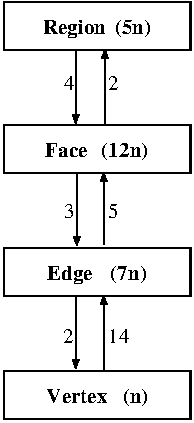
\includegraphics[scale=0.9]{figures/repF1} \\
        Representation F1
      \end{center}
    \end{minipage}
    \begin{minipage}{2.525in}
      \begin{center}
        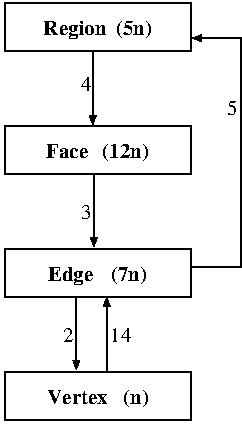
\includegraphics[scale=0.9]{figures/repF4} \\
        Representation F4
      \end{center}
    \end{minipage}
    \vspace{5em}

    \begin{minipage}{1.75in}
      \begin{center}
        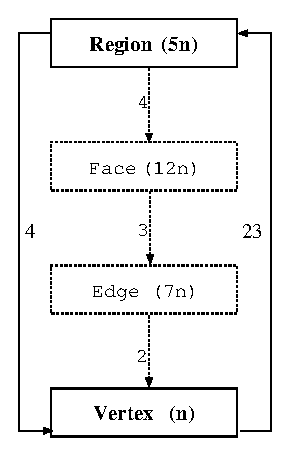
\includegraphics[scale=0.9]{figures/repR1} \\
        Representation R1
      \end{center}
    \end{minipage}
    \begin{minipage}{1.75in}
      \begin{center}
        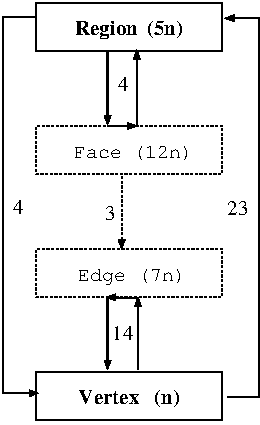
\includegraphics[scale=0.9]{figures/repR2} \\
        Representation R2
      \end{center}
    \end{minipage}
    \begin{minipage}{1.75in}
      \begin{center}
        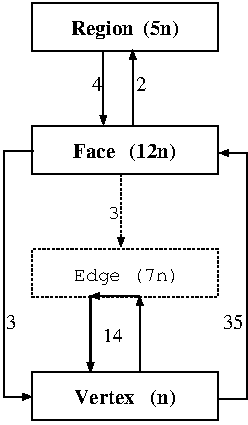
\includegraphics[scale=0.9]{figures/repR4} \\
        Representation R4
      \end{center}
    \end{minipage}
  \end{center}
  \caption{Mesh representations in MSTK}
  \label{fig:reptypes}
\end{figure}

\subsection{Volatile mesh entities in reduced representations}

As discussed above reduced representations, do not explicitly
represent all types of mesh entities. For example, R1 representations
do not explicitly represent edges and faces while R4 representations
do explicitly represent edges only. However, whenever an implicit
entity is requested from MSTK, the software creates a temporary entity
so that it appears that the entity actually exists in the
database. Since these entities are created-on-the-fly they are called
{\em volatile} mesh entities. For example, if an application asked for
the faces of a region in an R1 representation, MSTK will create as
many volatile faces as necessary, put them in a list and return them
to the calling application. Thus the application can pretend to work
with a full representation (although it is not always efficient to do so).

Volatile entities are stored for a period of time in internal data
structures in MSTK. Whenever there is a request for a new volatile
mesh entity, the code first checks if this entity has already been
created. If the volatile already exists in the database, then the
entity is returned as is and if it does not, it is created. This
ensures that many copies of the same entity are not created in
MSTK. However, to ensure that MSTK also does not store every volatile
entity forever (thereby, recreating a full representation), there is a
mechanism to perform garbage cleaning on volatile
entities. Periodically through the execution of the code, volatile
entities that have not been used for a long time are deleted from the
database freeing up valuable memory (which was the main point of using
a reduced representation after all).

To ensure that garbage cleaning does not delete a volatile mesh entity
that is being processed or stored by a calling application, MSTK also
provides a mechanism for locking entities. One can specify an autolock
mechanism for the entire mesh which means that no volatile entity will
ever be deleted once it is created. On the other hand, applications
may lock specific entities and unlock them when they cease to be
useful. 

\subsection{Mesh entity classification}

The concept of mesh entities of various dimensions is actually derived
from field of B-rep geometric modeling in which a model is comprised
of a hierarchy of topological entities of different dimensions. {\em
  Classification} is the relationship of each mesh entity to the model
entity is represents the whole or a part of.

To clarify further, every mesh is a discrete representation of a
geometric model. This geometric model may exist in the analyst's mind,
as schematic on paper or as a full model in a geometric modeling
system. Encoding the relationship of the mesh to this geometric model
to the extent possible provides enormous algorithmic benefits to the
users of meshes.

Recognizing that one may have varying degrees of information about the
geometric model in different situations, MSTK allows mesh entities to
store different levels of classification information or no
classification information.

Every mesh entity can store the dimension of the model entity it is on
({\bf GEntDim}), the ID of the model entity it is on ({\bf GEntID})
and a pointer to the model entity it is on ({\bf GEntity}). The
following picture illustrates the classification of various entities
in a simple mesh.

\begin{figure}
  \begin{center}
    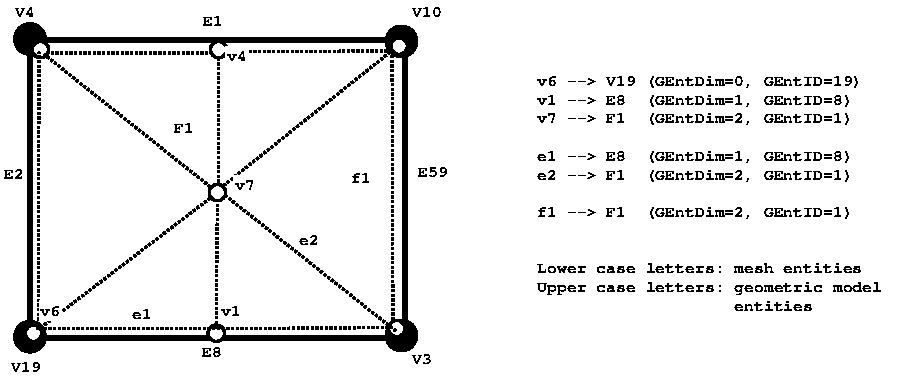
\includegraphics[width=\textwidth]{figures/classfn}
  \end{center}
  \caption{Example mesh and model showing the classification of mesh entities on geometric model entities}
\end{figure}

Classification information is very useful to have for simplifying
algorithms in meshing and analysis applications. For example, using
classification information, one can trivially extract all nodes on the
boundary and apply a different smoothing algorithm than nodes in the
interior of the domain. An FEA code can apply boundary conditions on
nodes and faces more easily if it has classification information.

If the application developer has nothing but the material IDs of the
mesh elements, MSTK can build the classification information to the
best of its ability using topological and geometric
information. However, it must be noted that this is procedure is not
perfect and some classification information cannot be derived
unambiguously. So, wherever possible, users are encouraged to generate
classification information during mesh generation and supply it to
MSTK.

\subsection{Parallel Mesh Management}

MSTK now has preliminary support for representation of distributed
surface and volume meshes for supporting parallel
simulations. \textit{This is an alpha functionality and the API or
  behavior of some functions is subject to revision.}

Currently, the only way to distribute meshes on multiple processors is
to perform a serial read on processor 0 and then distribute it to
however many processors are necessary. Mesh attributes and mesh entity
sets are appropriately partitioned and distributed to the different
processors. Functionality to read a pre-partitioned mesh is planned
for the future.

MSTK currently supports one (or no) layer of overlapped or ghost
entities between processors. If a surface mesh requests a layer of
ghost faces, then all lower order entities (edges and vertices)
forming the ghost faces are also ghosted. Similarly, if a volume mesh
requests a layer of ghost regions, all lower order entities (faces,
edges and vertices) forming the ghost regions are reproduced. Entities
that are owned by a processor but duplicated on another processor are
called {\em Overlap} entities. Entities that are duplicates of overlap
entities are called {\em Ghost} entities. The master processor ID of a
ghost entity is the processor ID that its corresponding overlap entity
lives on.

MSTK supports automatic updating of scalars, vectors and tensors on
mesh entities of all dimensions. The application can update the
attribute values on its owned entities and call MSTK to update the
attribute values on ghosts on other processors.

\textit{MSTK does not yet support parallel modification of meshes}.

\subsection{MSTK Application Programming Interface (API)}

Even though MSTK is written in C, MSTK is designed in an object
oriented manner. Mesh entities, mesh attributes and entity lists are
considered to be objects which have their private data and a set of
operators to query and manipulate this data. Even though methods may
be devised to circumvent the data hiding in MSTK, this is highly
discouraged. If you think that a particular operator is not efficient
or you don'thave access to some mesh data, please contact the
developer for assistance.

An important feature of MSTK is its ability to provide the full set of
mesh operators regardless of the representation used. When using
reduced representations, entities not represented explicitly in the
mesh are returned as volatile objects. However, it is possible to use
most MSTK operators on such objects as well.

Currently, MSTK offers only a C API but C++ and Fortran APIs are
planned for the near future.


\subsection{Getting meshes in and out of MSTK}

There are a few ways of getting mesh data into MSTK. The first is to
prepare an MSTK file with the full connectivity of an F1
representation and to read it in using MESH\_InitFromFile. This is
typically a difficult task for many applications which only have
element-node data. In such cases, one can prepare an MSTK file in the
R1 file format (in which the node listing is followed by the
region-node connectivity) and read it in to any of the other
representations, say F1. 

It is also possible to import meshes in other formats into MSTK. Some
formats that MSTK can read from are the GMV format and the ExodusII
format. Applications can use MESH\_ImportFromFile to import the mesh
into MSTK.

MSTK can write meshes out to different formats including GMV, STL and
ExodusII and FLAG X3D. When compiled with the appropriate options and
using a partitioner from an external library, MSTK can also write out
a parallel X3D file.

\newpage
\section{MSTK Data Types}

\begin{description}
\item[]{\bf {\em List\_ptr}}: Handle to a List object.

\item[]{\bf {\em Mesh\_ptr}}: Handle to a Mesh object.

\item[]{\bf {\em MVertex\_ptr}}: Handle to a Mesh Vertex object (Topological
Dimension 0).

\item[]{\bf {\em MEdge\_ptr}}: Handle to a Mesh Edge object (Topological Dimension 1).

\item[]{\bf {\em MFace\_ptr}}: Handle to a Mesh Face object (Topological Dimension 2).

\item[]{\bf {\em MRegion\_ptr}}: Handle to Mesh Region object (Topological Dimension 3).
  
\item[]{\bf {\em MEntity\_ptr}}: Handle to a generic Mesh Entity
  object. Any of the above types of entities can be cast as
  {\em MEntity\_ptr}.

\item[]{\bf {\em GModel\_ptr}}: Handle to a Geometric Model object.
\item[]{\bf {\em GEntity\_ptr}}: Handle to a Geometric Entity object.

\item[]{\bf {\em MAttrib\_ptr}}: Handle to a mesh attribute.
  
\item[]{\bf {\em RepType}}: Enumerated type describing the type
  of mesh representation.  Can be UNKNOWN\_REP, F1, F4, R1, R2, R4.
  See Appendix~\ref{fig:reptypes} for schematics of these
  representations. {\em Currently only representation types F1 and
    F4 are supported}.

\item[]{\bf {\em MType}}: Enumerated type for mesh entity type. Can be MDELETED, MVERTEX, MEDGE, MFACE, MREGION, MUNKNOWNTYPE, MALLTYPE.

\item[]{\bf {\em MFType}}: Enumerated type for mesh face type.
Can be FDELETED, FUNKNOWN, TRI, QUAD, POLYGON.

\item[]{\bf {\em MRType}}: Enumerated type for mesh region type.
Can be RDELETED, RUNKNOWN, TET, PYRAMID, PRISM, HEX, POLYHED.

\item[]{\bf {\em AttType}}: Enumerated type for attribute data. Can be INT, DOUBLE, POINTER, VECTOR or TENSOR.
\end{description}

\newpage
\section{MSTK Functional Interface}
\subsection{List}

Unordered lists of entities in MSTK are returned as type {\em
  List\_ptr} (See MSets for named entity sets). The following are the
list operations available in MSTK:

\begin{description}
\item[]{\bf {\em List\_ptr} List\_New({\em int} inisize):} Create a
new list with an initial size, {\em inisize}. If {\em inisize} is
0, the initial size is set to be 10.

\item[]{\bf {\em void} List\_Delete({\em List\_ptr} l):} Delete a list.
  
\item[]{\bf {\em List\_ptr} List\_Compress({\em List\_ptr}
    l):} Compress a list (delete all the null entries created when
  entities are removed from the list).  Doing this while an algorithm
  is iterating through the set can currently cause problems!! Calling
  {\bf List\_Compress} could change the pointer for the list due to
  reallocation.

\item[]{\bf {\em List\_ptr} List\_Copy({\em List\_ptr} l):} Return a
copy of a list.

\item[]{\bf {\em List\_ptr} List\_Add({\em List\_ptr} l, {\em void
  *}entry):} Add an entry to the list. The entry is strictly appended to the end
of the list.

\item[]{\bf {\em List\_ptr} List\_ChknAdd({\em List\_ptr} l,
{\em void *}entry):} Add an entry to a list only if it is not already
in the list.

\item[]{\bf {\em List\_ptr} List\_Insert({\em List\_ptr} l,
{\em void *}nuentry, {\em void *}b4entry):} Insert an entry into the list in the position before 'b4entry'.

\item[]{\bf {\em List\_ptr} List\_Inserti({\em List\_ptr} l,
    {\em void *}nuentry, {\em int} i):} Insert an entry into the
  list at the i'th valid position and push the entries previously at
  the i'th and later position back.

\item[]{\bf {\em int} List\_Rem({\em List\_ptr} l, {\em void
  *}entry):} Remove an entry from the list. Returns 1 if successful, 0
otherwise.

\item[]{\bf {\em int} List\_Remi({\em List\_ptr} l, {\em int} i):}
Remove the i'th valid entry in the list. Returns 1 if successful, 0
otherwise.

\item[]{\bf {\em int} List\_RemSorted({\em List\_ptr} l, {\em void}
    *entry, int (*entry2int)(void *)):} Remove an entry from a list
  that is sorted according to some correspondence between an entry and
  an integer value, e.g., {\bf MEnt\_ID(entry)} gives the ID of an
  entity. The mapping between the entry and the integer is given by a
  call to the routine {\bf entry2int}. The list could be one from which
  entities have previously been removed. The routine makes use of the
  sorted nature of the list to locate entries in $O(log(n))$ time
  where $n$ is the size of the list. An example call to this routine
  is

  \par {\bf fnd = List\_RemSorted(mregionslist,region,\&(MR\_ID));} 

\item[]{\bf {\em int} List\_Replace({\em List\_ptr} l, {\em void
  *}entry, {\em void *}nuentry):} Replace 'entry' with 'nuentry' in
set. Returns 1 if successful, 0 otherwise.

\item[]{\bf {\em int} List\_Replacei({\em List\_ptr} l, {\em int}
i, void *nuentry):} Replace the i'th valid entry in the list with
'nuentry'. Returns 1 if successful, 0 otherwise.

\item[]{\bf {\em int} List\_Contains({\em List\_ptr} l, void *entry):}
Returns 1 if list contains the entry, 0 otherwise.

\item[]{\bf {\em int} List\_Locate({\em List\_ptr} l, void *entry):}
Returns the positional index of the entry in the list. Returns -1 if
the list does not contain the entry.

\item[]{\bf {\em void *}List\_Entry({\em List\_ptr} l, {\em int}
i):} Return the i'th valid entry in the list.  Returns a NULL pointer if
the i'th valid entry could not be found.

\item[]{\bf {\em void *}List\_Next\_Entry({\em List\_ptr} l,
{\em int} *i):} Return the next valid entry in the list. This routine
works like an iterator. To start iterating through the list, set the
iteration index i=0 and call the routine to get the first entry in the
set. Subsequent calls to the routine will iterate through the entries
in the list. The routine will return a NULL to indicate that the end of
the set is reached.

The value of the iteration index i will be modified by the routine on
each call to indicate where in the list it is. This value should not be
modified externally while iterating through the list. Also, no specific
meaning should be derived from the iteration index by other applications
since the internal implementation and interpretation of the index may
change at any time.

Finally, there may be unexpected consequences if entries are removed
from the list while an iterator is iterating through it using {\bf
  List\_Next\_Entry}.

\item[]{\bf {\em int} List\_Num\_Entries({\em List\_ptr} l):} Return
the number of entries in a list.
\end{description}

\newpage
\subsection{Mesh Object}

A mesh object is a set of vertices (nodes) possibly connected by other
entities such as edges, faces, regions. Depending on the
representation chosen and type of mesh, some or all of the entities
may be explicitly stored.  Full representations contain all types of
entities up to the highest dimension of the mesh. For example, a full
representation of a tetrahedral mesh contains vertices, edges, faces
and regions. However, one type of reduced representation of this mesh
may contain only vertices and regions. For a surface mesh, a full
representation includes vertices, edges and faces while a reduced
representation only has vertices and faces. Also, depending on the
type of representation, some adjacencies (information about which
entities are connected to which other entities) are stored and others
are derived.

 
\begin{description}
\item[]{\bf {\em Mesh\_ptr} MESH\_New({\em RepType} type):}
  Initialize a new mesh object with the given representation type
  which can be F1, F2, F3, F4, F5, F6, R1, R2, R3, R4. Of these types
  F1, F4, R1, R2 and R4 are implemented. If the representation type is
  not known at the present time (e.g. before reading the mesh from a
  file), the representation type of UNKNOWN\_REP can be specified.
  Note that this only initializes a mesh object, it does not create or
  generate a mesh which is the work of high level mesh generation
  routines.

\item[]{\bf {\em int} MESH\_InitFromFile({\em Mesh\_ptr} mesh, const
    char *filename):} Initialize or read a mesh from a file in the
  MSTK format into the given mesh object. Returns 1 if successful, 0
  otherwise. It is possible to have a an MSTK file in the R1, R2 and
  R4 format into a mesh initialized as type F1 or F4. This routine
  imports any attributes that are into the mesh.

\item[]{\bf {\em int} MESH\_InitFromGenDesc({\em Mesh\_ptr} mesh, {\em
      int} nv, {\em double} (*xyz)[3], {\em int} nf, {\em int} *nfv, 
    {\em int} **fvids, {\em int} nr, {\em int} *nrv, {\em int}
    **rvids, {\em int} *nrf, {\em int} ***rfvtemplate):} Initialize a
  mesh from a
  minimal description of the mesh passed into the routine. In the
  routine, {\bf nv} is the number of vertices or nodes and {\bf xyz}
  is the array of node coordinates. If the mesh is a surface mesh,
  {\bf nf} is the number of mesh faces, {\bf nfv} gives the number of
  vertices for each face, {\bf fvids} gives the array indices of the
  face vertices in ccw manner (starting from 0, not 1). If the mesh is
  a solid mesh, {\bf nr} specifies the number of solid elements or
  regions. If the mesh has only standard element types (tets,
  pyramids, triangular prisms and hexes), then {\bf nrv} indicates the
  number of vertices of each region and {\bf rvids} gives the array
  indices of the region vertices. If, on the other hand, the mesh has
  polyhedral elements, regions have to be described in terms of faces
  which are in turn described in terms of vertices. Therefore, {\bf
    nrf} indicates the number of faces for each region and {\bf
    rfvtemplate} gives the array indices of the vertices for each face
  of the region.

\item[]{\bf {\em int} MESH\_ImportFromFile({\em Mesh\_ptr} mesh, const
    char *filename, const char *format):} Import a mesh data from an
  external file format and construct MSTK mesh. Currently the formats
  supported are the
  GMV\footnote{\texttt{http://www-xdiv.lanl.gov/XCM/gmv/GMVHome.html}}
  file format and the Exodus II file format. The routine imports as
  many attributes as it can from the input file. It also uses special
  attributes or keywords as data about element and node
  classification.  For GMV files, the routine uses the ``material''
  data to indicate region or face classification depending on the
  dimensionality of the mesh. If ``material'' data is not specified,
  it uses the ``itetclr'' attribute to assign region or face
  classification. It also uses the ``icr'' keyword describing the
  number of constraints on a node to interpret if the node is
  classified on a model region, model face, model edge or a model
  vertex. The ``itetclr'' and ``icr'' keywords are usually present in
  meshes generated by
  LAGRIT\footnote{\texttt{http://lagrit.lanl.gov}}. For Exodus II file
  formats, element blocks are used to create sets of mesh regions with
  the name 'matset\_N' (where N is the element block ID), sidesets are
  used to create sets of faces named 'sideset\_N' and nodesets are used
  to create sets of vertices named 'nodeset\_N'.

  
\item[]{\bf {\em int} MESH\_BuildClassfn({\em Mesh\_ptr} mesh):} Build
  classification information for mesh entities if only partial
  information is present. In other words, if the only data known is
  the IDs of geometric model entities (``material regions'') of the
  highest level mesh entities (faces or regions), then this procedure
  will build information about the type of geometric model entities
  that the lower dimension entities are on. Faces will be classified
  as being on a model face (external or interior) or inside model
  region. Edges will be classified as being on a model edge, model
  face or in a model region. Vertices will be classified as being on a
  model vertex, model edge, model face or in a model region. If no
  classification data is associated with even the highest level
  entities, the procedure will assume that all the highest level
  entities are classified on one model entitiy of that dimension. If
  partial information is available for lower order entities, this
  routine will not destroy that information. The procedure also tries
  to detect mesh edges that should be classified on model edges based
  on the fact that the dihedral angle between the boundary faces
  connected to the edge is smaller than some tolerance.



\item[]{\bf {\em int} MESH\_DelInterior({\em Mesh\_ptr}
    mesh):} Delete the interior of a mesh and retain only its
    boundaries (including interior boundaries). For solid meshes, this
    results in a surface mesh (i.e., all mesh regions, and  mesh
    faces, edges and vertices classified on model regions are deleted). For
    surface meshes, this results in curve mesh. For an edge mesh, only
    the end vertices are retained (unlikely to be used this
    way). Undefined for a vertex mesh.
  
  \item[]{\bf {\em void} MESH\_WriteToFile({\em Mesh\_ptr} mesh, const
      char *filename):} Save a mesh to a filename. The file is created
    if it does not exists. It is recommended that the .mstk extension
    be used for MSTK mesh files.  However, there is no such
    requirement. The routine will write out the mesh and any
    attributes attached to the mesh except attributes of the type
    POINTER.
  
  \item[]{\bf {\em void} MESH\_ExportToFile({\em Mesh\_ptr} mesh,
      const char *filname, const char *format, int natt, char
      **attnames):} Export a mesh to an external file
    format. Currently, the formats supported are the GMV file format
    (format: ``gmv'') and X3D (format: ``flag''), Exodus II file
    format (format: ``exodusii''). In addition surface meshes may be
    exported to STL (format: ``stl'') and IBM Data Explorer (format:
    ``dx'') format. Only integer and double attributes of the mesh are
    exported to GMV files and no attributes are exported to X3D files.

  \item[]{\bf {\em void} MESH\_ExportToGMV({\em Mesh\_ptr} mesh, const
      char *filname, int natt, char **attnames):} Export a mesh to a
    GMV file format.

\item[]{\bf {\em void} MESH\_ExportToFLAGX3D({\em Mesh\_ptr} mesh,
    const char *filname, int natt, char **attnames):} Export a mesh to
  the FLAG X3D format.

\item[]{\bf {\em void} MESH\_ExportToFLAGX3D\_Par({\em Mesh\_ptr}
    mesh, const char *filname, int natt, char **attnames, int
    *procids):} Export a mesh to the FLAG X3D format given a
  partitioned mesh. The owning processor for each element is given in
  the array {\bf procids}.

\item[]{\bf {\em void} MESH\_ExportToExodusII({\em Mesh\_ptr} mesh,
    const char *filname, int natt, char **attnames):} Export a mesh to
  a GMV file format.

\item[]{\bf {\em void} MESH\_ExportToDX({\em Mesh\_ptr} mesh, const
    char *filname):} Export a mesh to the IBM Data Explorer format
  (SURFACE MESHES ONLY!).

\item[]{\bf {\em void} MESH\_Tet2Hex({\em Mesh\_ptr} tetmesh, {\em
      Mesh\_ptr} *hexmesh):} Convert a tet mesh to a hex mesh by
  splitting the tets - the quality of the resulting hex mesh is
  usually not very good.

\item[]{\bf {\em void} MESH\_Renumber({\em Mesh\_ptr} mesh):} Renumber
  the entities of a mesh to avoid gaps in entity IDs. Note that in the
  current implementation, renumbering mesh entities can make removal
  of and searching for mesh entities much slower, so this must be
  avoided as much as possible.

\item[]{\bf {\em int} MESH\_PartitionWithMetis({\em Mesh\_ptr} mesh,
    {\em int} nparts, {\em int} **part):} Partition a mesh with the
  METIS libraries. 'part' is an array that contains the partition
  number for each mesh face (surface meshes) or mesh region (volume
  meshes). 

  \par {\bf NOTE THAT MSTK HAS TO HAVE BEEN COMPILED USING THE COMMAND
    'make PAR=1' AND THE CALLING APPLICATION MUST LINK WITH THE METIS
    LIBRARY.}

\item[]

\item[]{\bf {\em GModel\_ptr} MESH\_GModel({\em Mesh\_ptr} mesh):}
Return a handle to the underlying geometric model. If there is no
geometric model associated with the mesh, NULL pointer is returned.

\item[]{\bf {\em RepType} MESH\_RepType({\em Mesh\_ptr} mesh):}
Representation type currently being used by the mesh.

\item[]{\bf {\em char } *MESH\_RepType({\em Mesh\_ptr} mesh):}
  Representation type currently being used by the mesh returned as a
  2-character string.

\item[]

\item[]{\bf {\em int} MESH\_Num\_Vertices({\em Mesh\_ptr} mesh):}
Number of vertices in the mesh. This includes owned and ghost
vertices.

\item[]{\bf {\em int} MESH\_Num\_Edges({\em Mesh\_ptr} mesh):} Number
  of edges in the mesh (owned and ghost). For reduced representations,
  this routine returns 0 since it is impractically expensive to count
  the number of edges when they do not explicitly exist. Applications
  must find a way to avoid using this routine for reduced
  representations.

\item[]{\bf {\em int} MESH\_Num\_Faces({\em Mesh\_ptr} mesh):} Number
  of faces in the mesh (owned and ghost). For reduced representations
  R1 or R2, this routine counts only the faces that are explicitly
  represented i.e. faces not connected to any mesh region. Therefore,
  a value of 0 will be returned for the number of faces of a
  tetrahedral mesh with representation R1 or R2 but the correct number
  will be reported for a tetrahedral mesh in other
  representations. Also, the correct number will be reported for the
  number of faces in a surface mesh in representation R1 or R2.
  Therefore, this routine must be used carefully.


\item[]{\bf {\em int} MESH\_Num\_Regions({\em Mesh\_ptr} mesh):}
Number of regions in the mesh (owned and ghost).

\item[]

\item[]{\bf {\em MVertex\_ptr} MESH\_Vertex({\em Mesh\_ptr} mesh,
{\em int} i):} Return the i'th vertex in the mesh. Returns NULL if i
$<$ 0 or i $>$ number of mesh vertices. The vertex may be owned or ghost.

\item[]{\bf {\em MEdge\_ptr} MESH\_Edge({\em Mesh\_ptr} mesh, {\em
    int} i):} Return the i'th edge in the mesh. Returns NULL if i $<$
  0 or i $>$ number of mesh edges. The edge may be owned or
  ghost. Returns NULL for reduced representations.

\item[]{\bf {\em MFace\_ptr} MESH\_Face({\em Mesh\_ptr} mesh, {\em
    int} i):} Return the i'th face in the mesh. Returns NULL if i $<$
  0 or i $>$ number of mesh faces. The face may be owned or
  ghost. Only faces explicitly represented in the mesh are returned
  for reduced representation (See explanation for MESH\_Num\_Faces).

\item[]{\bf {\em MRegion\_ptr} MESH\_Region({\em Mesh\_ptr} mesh, {\em
    int} i):} Return the i'th region in the mesh. Returns NULL if i
  $<$ 0 or i $>$ number of mesh region. The region may be owned or
  ghost.

\item[]

\item[]{\bf {\em MVertex\_ptr} MESH\_Next\_Vertex({\em Mesh\_ptr}
  mesh, {\em int} *idx):} Returns the next vertex while iterating
  through the vertices of the mesh. The vertex may be owned or ghost
  and the type must be checked using {\bf MV\_PType}. See the routine
  {\bf List\_Next\_Entry} above for an explanation of how the
  iteration works. This routine is in general faster than using the
  routine {\bf MESH\_Vertex}.

\item[]{\bf {\em MEdge\_ptr} MESH\_Next\_Edge({\em Mesh\_ptr} mesh,
  {\em int} *idx):} Returns the next edge while iterating through the
  edges of the mesh. The edge may be owned or ghost
  and the type must be checked using {\bf ME\_PType}. See the routine
  List\_Next\_Entry above for an explanation of how the iteration
  works.  The routine always returns NULL for reduced representations.

\item[]{\bf {\em MFace\_ptr} MESH\_Next\_Face({\em Mesh\_ptr} mesh,
  {\em int} *idx):} Returns the next face while iterating through the
  faces of the mesh. The face may be owned or ghost
  and the type must be checked using {\bf MF\_PType}. See the routine
  {\bf List\_Next\_Entry} above for an explanation of how the
  iteration works.  Only faces explicitly represented in the mesh are
  returned for reduced representation (See explanation for {\bf
    MESH\_Num\_Faces}).

\item[]{\bf {\em MRegion\_ptr} MESH\_Next\_Region({\em Mesh\_ptr}
  mesh, {\em int} *idx):} Returns the next region while iterating
  through the regions of the mesh. The region may be owned or ghost
  and the type must be checked using {\bf MR\_PType}. See the routine
  {\bf List\_Next\_Entry} above for an explanation of how the
  iteration works.
  
\item[]

\item[]{\bf {\em MVertex\_ptr}
    MESH\_VertexFromID({\em Mesh\_ptr} mesh, {\em int} id):}
  Return mesh vertex with given ID if it exists; return NULL
  otherwise.
  
\item[]{\bf {\em MEdge\_ptr} MESH\_EdgeFromID({\em Mesh\_ptr}
    mesh, {\em int} id):} Return mesh edge with given ID if it
  exists; return NULL otherwise. This routine will return NULL for all
  reduced representations.

\item[]{\bf {\em MFace\_ptr} MESH\_FaceFromID({\em Mesh\_ptr}
    mesh, {\em int} i):} Return mesh face with given ID if it
  exists; return NULL otherwise. If faces are not explicitly
  represented in the mesh, it will return NULL.


\item[]{\bf {\em MRegion\_ptr}
    MESH\_RegionFromID({\em Mesh\_ptr} mesh, {\em int} id):}
  Return mesh region with given ID if it exists; return NULL
  otherwise.

\item[]{\bf {\em MEntity\_ptr} MESH\_EntityFromID({\em Mesh\_ptr}
    mesh, {\em MType mtype}, {\em int} id):} Return mesh entity of
  given type and given ID if it exists; return NULL otherwise.

\item[]

\item[]{\bf {\em int} MESH\_Num\_Attribs({\em Mesh\_ptr}
    mesh):} Number of attributes associated with the mesh.
  
\item[]{\bf {\em MAttrib\_ptr} MESH\_Attrib({\em Mesh\_ptr}
    mesh, {\em int} i):} Return the i'th attribute in the mesh.
  Returns NULL if i $<$ 0 or i $>$ number of mesh attributes.
 
\item[]{\bf {\em MAttrib\_ptr}
    MESH\_Next\_Attrib({\em Mesh\_ptr} mesh, {\em int} *index):}
  Returns the next attribute while iterating through the attributes of
  the mesh. See the routine List\_Next\_Entry above for an explanation
  of how the iteration works.
  
\item[]{\bf {\em MAttrib\_ptr}
    MESH\_AttribByName({\em Mesh\_ptr} mesh, {\em const char}
    *name):} Return a mesh attribute with given name if it exists in
  the mesh. Returns NULL if mesh has no such attribute.

\item[]
  
\item[]{\bf {\em int} MESH\_Num\_MSets({\em Mesh\_ptr}
    mesh):} Number of entity sets associated with the mesh.
  
\item[]{\bf {\em MSet\_ptr} MESH\_MSet({\em Mesh\_ptr}
    mesh, {\em int} i):} Return the i'th entity set in the mesh.
  Returns NULL if i $<$ 0 or i $>$ number of entity sets.
 
\item[]{\bf {\em MSet\_ptr}
    MESH\_Next\_MSet({\em Mesh\_ptr} mesh, {\em int} *index):}
  Returns the next entity set while iterating through the sets of
  the mesh. See the routine List\_Next\_Entry above for an explanation
  of how the iteration works.
  
\item[]{\bf {\em MSet\_ptr}
    MESH\_MSetByName({\em Mesh\_ptr} mesh, {\em const char}
    *name):} Return a mesh entity set with given name if it exists in
  the mesh. Returns NULL if mesh has no such set.

\item[]
  

\item[]{\bf {\em void} MESH\_Set\_GModel({\em Mesh\_ptr} mesh,
GModel\_ptr geom):} Assign a geometric model handle to the mesh.

%\item[]{\bf {\em int} MESH\_Change\_RepType({\em Mesh\_ptr} mesh,
%{\em int} nurep):} Change the representation type of the mesh. This
%routine can be used to modify the representation type dynamically to
%suit different algorithms.  However, the cost of making the change and
%reordering all adjacencies and creating or deleting entities has to be
%considered while invoking this routine. Also, once a conversion is
%made from a full representation to a reduced representation, not all
%information may be retrievable when switching back to a full
%representation.  (particularly classification information, i.e.,
%relationship of mesh entities to the geometric model).

\item[]

\item[]{\bf {\em void} MESH\_Add\_Vertex({\em Mesh\_ptr}
    mesh, {\em MVertex\_ptr} v):} Add a vertex to the mesh. It is
  assumed that the vertex and its coordinates set are properly
  defined. Normally, one need not call this since
  {\bf {\em MV\_New}} will add the vertex to the mesh. Use this
  only if you know exactly what you are doing.

\item[]{\bf {\em void} MESH\_Add\_Edge({\em Mesh\_ptr} mesh,
    {\em MEdge\_ptr} e):} Add an edge to the mesh. It is assumed
  that the edge is and its topology is defined. Normally, one need not
  call this since {\bf {\em ME\_New}} will add the edge to the
  mesh. Use this only if you know exactly what you are doing.

\item[]{\bf {\em void} MESH\_Add\_Face({\em Mesh\_ptr} mesh,
    {\em MFace\_ptr} f):} Add a face to the mesh. It is assumed
  that the face and its topology is properly defined. Normally, one
  need not call this since {\bf {\em MF\_New}} will add the face
  to the mesh. Use this only if you know exactly what you are doing.

\item[]{\bf {\em void} MESH\_Add\_Region({\em Mesh\_ptr}
    mesh, {\em MRegion\_ptr} r):} Add a region to the mesh. It is
  assumed that the region and its topology is properly defined.
  Normally, one need not call this since {\bf {\em MR\_New}}
  will add the region to the mesh. Use this only if you know exactly
  what you are doing.

\item[]{\bf {\em void} MESH\_Rem\_Vertex({\em Mesh\_ptr}
    mesh, {\em MVertex\_ptr} v):} Remove vertex from mesh. Vertex
  is not deleted and must be deleted afterward separately. Normally,
  one need not call this since {\bf {\em MV\_Delete}} will
  remove the vertex from the mesh. Use this only if you know exactly
  what you are doing.

\item[]{\bf {\em void} MESH\_Rem\_Edge({\em Mesh\_ptr} mesh,
    {\em MEdge\_ptr} e):} Remove edge from mesh. Edge is not
  deleted and must be deleted afterward separately. Normally, one need
  not call this since {\bf {\em ME\_Delete}} will remove the
  edge from the mesh. Use this only if you know exactly what you are
  doing.
  
\item[]{\bf {\em void} MESH\_Rem\_Face({\em Mesh\_ptr} mesh,
    {\em MFace\_ptr} f):} Remove face from mesh. Face is not
  deleted and must be deleted afterward separately. Normally, one need
  not call this since {\bf {\em MF\_Delete}} will remove the
  face from the mesh. Use this only if you know exactly what you are
  doing.
  
\item[]{\bf {\em void} MESH\_Rem\_Region({\em Mesh\_ptr}
    mesh, {\em MRegion\_ptr} r):} Remove region from mesh. Region
  is not deleted and must be deleted afterward separately. Normally,
  one need not call this since {\bf {\em MR\_Delete}} will
  remove the region from the mesh. Use this only if you know exactly
  what you are doing.


\item[]{\bf {\em void} MESH\_Set\_AutoLock({\em Mesh\_ptr} mesh, {\em
      int} autolock):} If autolock is 1, all volatile mesh entities
  created in reduced representations will be automatically locked and
  cannot be removed by garbage cleaning procedures (They can still be
  removed by explicitly calling a delete on them). If it 0, volatile
  mesh entities can be deleted internally after a period of disuse.

\item[]{\bf {\em int} MESH\_AutoLock({\em Mesh\_ptr} mesh):} Return
the autolock status for volatile entities (See {\bf
  MESH\_Set\_AutoLock} for details).

\end{description}

\newpage
\subsection{Mesh Vertex Object}

\begin{description}
\item[]{\bf {\em MVertex\_ptr} MV\_New({\em Mesh\_ptr}
    mesh):} Create a new vertex object. No geometric or topological
  information is embedded in the vertex when it is created. The vertex
  only knows which mesh it belongs to. The ID of the vertex is set by
  this function.
  
\item[]{\bf {\em void} MV\_Delete({\em MVertex\_ptr} mvertex,
    {\em int} keep):} Delete the vertex. If {\bf keep} is 0, the
  vertex is removed from the mesh and all topological and geometric
  information embedded in the vertex is destroyed. If {\bf keep} is
  1, the vertex is marked as type {\em MDELVERTEX} and removed from
  the mesh but the vertex is not destroyed.


  \par {\bf NOTE: {\em MV\_Delete} AND ITS COUNTERPARTS WILL, IN GENERAL,
    REMOVE AN ENTITY IN $O(log(N))$ TIME WHERE $N$ IS THE TOTAL NUMBER
    OF ENTITIES ADDED TO THE MESH SINCE THE START OF THE
    PROGRAM. HOWEVER, IF THE MESH ENTITIES HAVE NOT BEEN RENUUMBERED
    (EITHER USING MESH\_RENUMBER OR EXPLICITLY USING MENT\_SET\_ID) OR
    THE MESH ENTITY LISTS HAVE NOT BEEN COMPRESSED THEN THE REMOVAL
    TIME IS $O(1)$ WHICH IS CLEARLY MUCH SUPERIOR.}


\item[]{\bf {\em void} MV\_Restore({\em MVertex\_ptr}
    mvertex):} Restore a deleted vertex. The vertex type is restored
  from {\em MDELVERTEX} to {\em MVERTEX} and the vertex is
  added back to the mesh.

\item[]
  
\item[]{\bf {\em void} MV\_Set\_Coords({\em MVertex\_ptr}
    mvertex, double *xyz):} Set the coordinates of the vertex.
    
\item[]{\bf {\em void} MV\_Set\_GEntity({\em MVertex\_ptr}
    mvertex, GEntity\_ptr gent):} Set the geometric model entity on
  which vertex is classified.


\item[]{\bf {\em void} MV\_Set\_GEntDim({\em MVertex\_ptr} mvertex,
{\em int} gdim):} Set topological dimension of model entity on which
vertex is classified.

\item[]{\bf {\em void} MV\_Set\_GEntID({\em MVertex\_ptr} mvertex,
{\em int} gid):} Set ID of model entity on which vertex is
classified.

\item[]{\bf {\em void} MV\_Add\_AdjVertex({\em MVertex\_ptr}
mvertex, {\em MVertex\_ptr} adjvertex):} Add neighboring vertex,
adjvertex, to ajdacent vertex list of vertex, mvertex.

\item[]{\bf {\em void} MV\_Rem\_AdjVertex({\em MVertex\_ptr}
mvertex, {\em MVertex\_ptr} adjvertex):} Delete neighboring vertex
of given vertex.

\item[]{\bf {\em void} MV\_Set\_ID({\em MVertex\_ptr} mvertex,
{\em int} id):} Explicitly set ID of a vertex and overwrite the ID
set by the MV\_New operator. Does not check for duplication of edge
IDs.

\item[]

\item[]{\bf {\em Mesh\_ptr} MV\_Mesh({\em MVertex\_ptr} mv):}
Returns the mesh that this vertex belongs to.

\item[]{\bf {\em int} MV\_ID({\em MVertex\_ptr} mvertex):} Returns
the ID of the vertex. 

\item[]{\bf {\em int} MV\_GEntDim({\em MVertex\_ptr} mvertex):}
Returns the dimension of the geometric model entity that the vertex is
classified on. Returns -1 if not known.

\item[]{\bf {\em int} MV\_GEntID({\em MVertex\_ptr} mvertex):}
Returns the ID of the geometric model entity that the vertex is
classified on. Returns 0 if this information is not known.

\item[]{\bf {\em GEntity\_ptr} MV\_GEntity({\em MVertex\_ptr}
  mvertex):} Returns a pointer or handle to the geometric model entity
  that the vertex is classified on. Returns NULL if this information
  is not known.

\item[]{\bf {\em void} MV\_Coords({\em MVertex\_ptr} mvertex,
double *xyz):} Returns the coordinates of the vertex.

\item[]

\item[]{\bf {\em int} MV\_Num\_AdjVertices({\em MVertex\_ptr}
mvertex):} Returns the number of edge connected neighboring vertices of
vertex. {\em Not efficient for all representations}.

\item[]{\bf {\em int} MV\_Num\_Edges({\em MVertex\_ptr} mvertex):}
Returns the number of edges connected to the vertex.

\item[]{\bf {\em int} MV\_Num\_Faces({\em MVertex\_ptr} mvertex):}
Returns the number of faces connected to the vertex.

\item[]{\bf {\em int} MV\_Num\_Regions({\em MVertex\_ptr} mvertex):}
Returns the number of regions connected to the vertex

\item[]{\bf {\em List\_ptr} MV\_AdjVertices({\em MVertex\_ptr}
mvertex):} List of adjacent or edge connected neighboring vertices of vertex.

\item[]{\bf {\em List\_ptr} MV\_Edges({\em MVertex\_ptr} mvertex):}
List of edges connected to the vertex. {\bf The list returned by this
  operator must be deleted by the calling application using {\em List\_Delete}}.

\item[]{\bf {\em List\_ptr} MV\_Faces({\em MVertex\_ptr} mvertex):}
List of faces connected to the vertex. {\bf The list returned by this
  operator must be deleted by the calling application using {\em List\_Delete}}.

\item[]{\bf {\em List\_ptr} MV\_Regions({\em MVertex\_ptr} mvertex):}
List of regions connected to the vertex. {\bf The list returned by this
  operator must be deleted by the calling application using {\em List\_Delete}}.

\item[]

\item[]  {\bf {\em PType} MV\_PType({\em MVertex\_ptr} v)}: Parallel entity type for vertex - can be PINTERIOR, POVERLAP or PGHOST.
\item[]  {\bf {\em int}   MV\_MasterParID({\em MVertex\_ptr} v)}:
\item[]  {\bf {\em int}   MV\_GlobalID({\em MVertex\_ptr} v)}:

\item[]
\item[]  The following three functions affect how mesh entities communicate and how their attributes are updated. IF YOU DON'T KNOW WHAT YOU ARE DOING WHEN YOU CALL THIS FUNCTION, YOU WILL GET WHAT YOU DESERVE.
\item[]  {\bf {\em void}  MV\_Set\_PType({\em MVertex\_ptr} v, {\em PType} ptype)}: 
\item[]  {\bf {\em void}  MV\_Set\_MasterParID({\em MVertex\_ptr} v, {\em int} masterparid)}
\item[]  {\bf {\em void}  MV\_Set\_GlobalID({\em MVertex\_ptr} v, {\em int} globalid)}:  


\end{description}



\newpage
\subsection{Mesh Edge Object}

\begin{description}
\item[]{\bf {\em MEdge\_ptr} ME\_New({\em Mesh\_ptr} mesh):}
  Create a new edge object. No topological information is embedded in
  the edge when it is created. The edge only knows which mesh it
  belongs to. The ID of the edge is set by this function.
  
\item[]{\bf {\em void} ME\_Delete({\em MEdge\_ptr} medge,
    {\em int} keep):} Delete the edge. If {\bf keep} is 0, the
  edge is removed from the mesh and all topological and geometric
  information embedded in the edge is destroyed. If {\bf keep} is
  1, the edge is marked as type {\em MDELEDGE} and removed from the
  mesh but the edge is not destroyed. Also, the vertices of this edge
  no longer point to this edge.
    
\item[]{\bf {\em void} ME\_Restore({\em MEdge\_ptr}
    medge):} Restore a temporarily deleted edge. The edge type is
  restored from {\em MDELEDGE} to {\em MEDGE} and the edge is
  added back to the mesh. The vertices of the edge once again point
  back to the edge.

\item[]
  
\item[]{\bf {\em void} ME\_Set\_GEntity({\em MEdge\_ptr}
    medge, GEntity\_ptr gent):} Set the geometric model entity on
  which the edge is classified.
  
\item[]{\bf {\em void} ME\_Set\_GEntDim({\em MEdge\_ptr}
    medge, {\em int} gdim):} Set the topological dimension of model
  entity on which edge is classified.
  
\item[]{\bf {\em void} ME\_Set\_GEntID({\em MEdge\_ptr}
    medge, {\em int} gid):} Set ID of model entity on which edge is
  classified.
  
\item[]{\bf {\em void} ME\_Set\_GInfo\_Auto({\em MEdge\_ptr} medge):}
  Derive the classification (GEntDim, GEntID) of the mesh edge
  automatically (if possible) from the classification of its
  vertices. If it is not possible to unambiguously get this
  information, the procedure will keep the default information. {\bf THIS
  MAY GET WRONG OR INCORRECT INFORMATION WHEN THERE IS AMBIGUOUS
  DATA. FOR EXAMPLE, IF THE VERTICES OF A MESH EDGE ARE CLASSIFIED ON
  TWO DIFFERENT MODEL VERTICES, IT IS NOT POSSIBLE TO KNOW WHAT ENTITY
  THE MESH EDGE IS CLASSIFIED USING JUST THE VERTEX INFORMATION.}

\item[]{\bf {\em void} ME\_Set\_ID({\em MEdge\_ptr} medge,
    {\em int} id):} Explicitly set ID of an edge and overwrite the
  ID set by the ME\_New function. Does not check for duplication of
  edge IDs.
  
\item[]{\bf {\em void} ME\_Set\_Vertex({\em MEdge\_ptr}
    medge, {\em int} i, {\em MVertex\_ptr} vertex):} Set the
  i'th vertex of the edge. i can be 0 or 1.
  
\item[]{\bf {\em void} ME\_Replace\_Vertex({\em MEdge\_ptr}
    medge, {\em MVertex\_ptr} vert, {\em MVertex\_ptr} nuvert):}
  Replace i'th vertex by new vertex.

\item[]
  
\item[]{\bf {\em Mesh\_ptr} ME\_Mesh({\em MEdge\_ptr}
    medge):} Returns the mesh that this edge belongs to.
  
\item[]{\bf {\em int} ME\_ID({\em MEdge\_ptr} medge):}
  Returns the ID of the vertex. Returns -1 if not known.
  
\item[]{\bf {\em int} ME\_GEntDim({\em MEdge\_ptr} medge):}
  Returns the dimension of the geometric model entity that the vertex
  is classified on. Returns -1 if not known.
  
\item[]{\bf {\em int} ME\_GEntID({\em MEdge\_ptr} medge):}
  Returns the ID of the geometric model entity that the vertex is
  classified on.  Returns 0 if this information is not known.
  
\item[]{\bf {\em GEntity\_ptr} ME\_GEntity({\em MEdge\_ptr}
    medge):} Returns a pointer or handle to the geometric model entity
  that the vertex is classified on. Returns NULL if this information
  is not known.

\item[]
  
\item[]{\bf {\em int} ME\_Num\_Faces({\em MEdge\_ptr}
    medge):} Returns the number of faces connected to the edge.
  
\item[]{\bf {\em int} ME\_Num\_Regions({\em MEdge\_ptr}
    medge):} Returns the number of regions connected to the edge.
  
\item[]{\bf {\em MVertex\_ptr} ME\_Vertex({\em MEdge\_ptr}
    medge, {\em int} i):} Returns the i'th vertex of the edge. i=0
  returns the first vertex and i=1 returns the second vertex.
  
\item[]{\bf {\em MVertex\_ptr} ME\_OppVertex({\em MEdge\_ptr}
    medge, {\em MVertex\_ptr} ov):} Return the vertex opposite to
  given vertex in edge.
  
\item[]{\bf {\em int} ME\_UsesEntity({\em MEdge\_ptr} medge,
    {\em MEntity\_ptr} mentity, {\em int} etype):} Check if edge
  uses given lower dimension entity, {\em mentity}. The dimension
  of the entity is specified by the {\em etype} variable. For an
  edge, the only lower dimensional entity is a vertex. If the edge
  uses the vertex, the function returns 1; otherwise it returns 0. If
  any other type of entity is specified, the function returns 0.

  
\item[]{\bf {\em List\_ptr} ME\_Faces({\em MEdge\_ptr}
    medge):} Returns the set of faces using this edge. {\bf The list returned by this
  operator must be deleted by the calling application using {\em List\_Delete}}.
  
\item[]{\bf {\em List\_ptr} ME\_Regions({\em MEdge\_ptr}
    medge):} Returns the set of regions using this edge. {\bf The list returned by this
  operator must be deleted by the calling application using {\em List\_Delete}}.

\item[]
  
\item[]{\bf {\em MEdge\_ptr}
    MVs\_CommonEdge({\em MVertex\_ptr} v1, {\em MVertex\_ptr}
    v2):} Return the edge connecting vertices v1 and v2, if it exists.
  If such an edge does not exist, the function returns 0.
  
\item[]{\bf {\em double} ME\_Len({\em MEdge\_ptr} e):} Return
  the length of the straight line connecting the two vertices of the
  edge.
  
\item[]{\bf {\em double} ME\_LenSqr({\em MEdge\_ptr} e):}
  Return the square of the length of the straight line connecting the
  two vertices of the edge.
  
\item[]{\bf {\em void} ME\_Vec({\em MEdge\_ptr} e, double
    *evec):} Return the vector going from the first vertex of the edge
  to the second vertex of the edge.

\item[]{\bf {\em int} MEs\_AreSame({\em MEdge\_ptr} e1, {\em
      MEdge\_ptr} e2):} {\em Applicable only to reduced
    representations.} Check if two edges described by only their
  vertices are the same. In a reduced representation, edges are
  temporary objects described by their end vertices. If two temporary
  edges are described by the same vertices, the edges are considered
  to be the same.

\item[]

\item[]{\bf {\em void} ME\_Lock({\em MEdge\_ptr} e):} Lock a volatile
  edge so that it cannot be deleted by garbage cleaning procedures (It
  can still be deleted by {\bf ME\_Delete}.

\item[]{\bf {\em void} ME\_UnLock({\em MEdge\_ptr} e):} Unlock a volatile
  edge so that it may be deleted freely by garbage cleaning procedures.

\item[]

\item[]  {\bf {\em PType} ME\_PType({\em MEdge\_ptr} v)}: Parallel entity type for edge - can be PINTERIOR, POVERLAP or PGHOST.
\item[]  {\bf {\em int}   ME\_MasterParID({\em MEdge\_ptr} v)}:
\item[]  {\bf {\em int}   ME\_GlobalID({\em MEdge\_ptr} v)}:

\item[]
\item[]  The following three functions affect how mesh entities communicate and how their attributes are updated. IF YOU DON'T KNOW WHAT YOU ARE DOING WHEN YOU CALL THIS FUNCTION, YOU WILL GET WHAT YOU DESERVE.
\item[]  {\bf {\em void}  ME\_Set\_PType({\em MEdge\_ptr} v, {\em PType} ptype)}: 
\item[]  {\bf {\em void}  ME\_Set\_MasterParID({\em MEdge\_ptr} v, {\em int} masterparid)}
\item[]  {\bf {\em void}  ME\_Set\_GlobalID({\em MEdge\_ptr} v, {\em int} globalid)}:  


\end{description}



\newpage
\subsection{Mesh Face Object}

\begin{description}
\item[]{\bf {\em MFace\_ptr} MF\_New({\em Mesh\_ptr} mesh):} Create
a new face object. No topological information is embedded in the face
when it is created. The face only knows which mesh it belongs
to. The ID of the face is set by this function.

\item[]{\bf {\em void} MF\_Delete({\em MFace\_ptr} mface):}
  Delete the face. If {\bf keep} is 0, the face is removed from the
  mesh and all topological and geometric information embedded in the
  face is destroyed. If {\bf keep} is 1, the face is marked as type
  {\em MDELFACE} and removed from the mesh but the face is not
  destroyed. Also, the vertices/edges of this face no longer point up
  to this face.
    
\item[]{\bf {\em void} MF\_Restore({\em MFace\_ptr}
    mface):} Restore a temporarily deleted face. The face type is
  restored from {\em MDELFACE} to {\em MFACE} and the face is
  added back to the mesh. The vertices/edges of the face once again point
  back to the face.

\item[]
  
\item[]{\bf {\em void} MF\_Set\_GEntity({\em MFace\_ptr} mface, GEntity\_ptr gent):} Set the geometric model entity on which the face is classified.

\item[]{\bf {\em void} MF\_Set\_GEntDim({\em MFace\_ptr} mface,
{\em int} gdim):} Set the dimension of the geometric model entity on
which the face is classified.

\item[]{\bf {\em void} MF\_Set\_GEntID({\em MFace\_ptr} mface,
{\em int} gid):} Set the ID of the geometric model entity on which
the face is classified.

\item[]{\bf {\em void} MF\_Set\_GInfo\_Auto({\em MFace\_ptr} mface):}
  Derive the classification (GEntDim, GEntID) of the mesh face
  automatically (if possible) from the classification of its
  vertices or edges. If it is not possible to unambiguously get this
  information, the procedure will keep the default information. {\bf THIS
  MAY GET WRONG OR INCORRECT INFORMATION WHEN THERE IS AMBIGUOUS
  DATA.}


\item[]{\bf {\em void} MF\_Set\_ID({\em MFace\_ptr} mface,
{\em int} id):} Explicitly set ID of a face and overwrite the ID
set by the {\bf MF\_New} operator. Does not check for duplication of face
IDs.

\item[]{\bf {\em void} MF\_Set\_Edges({\em MFace\_ptr} mface,
{\em int} n, {\em MEdge\_ptr} *edges, {\em int} *dirs):} Set
the edges of the face along with their directions. The ordered set of
edge pointers and their directions are passed in through arrays along
with the number of edges. The edges are assumed to be ordered
clockwise around the face. If an edge direction is along the clockwise
direction of the face then the entry in the 'dirs' array must be 1;
otherwise it must be 0. This function is relevant only for full
representations in MSTK.

\item[]{\bf {\em void} MF\_Set\_Vertices({\em MFace\_ptr}
    mface, {\em int} n, {\em MVertex\_ptr} *verts):} Set the
  vertices of the face. The ordered set of vertices (ccw around the
  face) is passed in through an array along with the number of
  vertices. This routine will collect/build all lower order
  topological information (edges, edge directions in the face) as needed by the face.
  
\item[]{\bf {\em void} MF\_Replace\_Edges({\em MFace\_ptr} mface, {\em
      int} nold, {\em MEdge\_ptr} *oldedges, {\em int} nnu, {\em
      MEdge\_ptr} *nuedges):} Replace a set of edges in the face with
  another set of edges. The direction in which the new edges are to be
  used in the face are automatically deduced.  This function is
  relevant only for full representations in MSTK. The old and new edge
  sets must be comprised of edges connected to each other and the end
  vertices of the new set must match the end vertices of the new set.
  
\item[]{\bf {\em void} MF\_Replace\_Edges\_i({\em MFace\_ptr}
    mface, {\em int} nold, {\em int} i, {\em int} nnu,
    {\em MEdge\_ptr} *nuedges):} Replace the {\em nold} edges in
  the face starting with the i'th edge and going ccw around the face
  with a new set of edges. The directions in which the new edges are
  used in the face are automatically deduced. This function is
  relevant only for full representations in MSTK.

\item[]{\bf {\em void} MF\_Replace\_Vertex({\em MFace\_ptr} mface,
{\em MVertex\_ptr} mvertex, {\em MVertex\_ptr} nuvertex):}
Replace a vertex in the face with another vertex. This function is
relevant only for reduced representations in MSTK.

\item[]{\bf {\em void} MF\_Replace\_Vertex\_i({\em MFace\_ptr}
mface, {\em int} i, {\em MVertex\_ptr} nuvertex):} Replace the
i'th vertex in the face with a new vertex. This function is relevant
only for reduced representations in MSTK.

\item[]{\bf {\em void} MF\_Insert\_Vertex({\em MFace\_ptr} mface,
{\em MVertex\_ptr} nuvertex, {\em MVertex\_ptr} b4vertex):}
Insert a vertex in the face before {\bf b4vertex} w.r.t. a ccw
ordering of the vertex faces. 

\item[]{\bf {\em void} MF\_Insert\_Vertex\_i({\em MFace\_ptr}
mface, {\em MVertex\_ptr} nuvertex, {\em int} i):} Insert a new
vertex before vertex i in the face w.r.t. a ccw ordering of vertices.

\item[]

\item[]{\bf {\em Mesh\_ptr} MF\_Mesh({\em MFace\_ptr} mf):} Returns the mesh that this mesh belongs to.

\item[]{\bf {\em int} MF\_ID({\em MFace\_ptr} mface):} Returns the ID of the face. Returns 0 if not known.

\item[]{\bf {\em int} MF\_GEntDim({\em MFace\_ptr} mface):} Returns the dimensions of the geometric model entity that the vertex is classified on. Returns -1 if not known.

\item[]{\bf {\em int} MF\_GEntID({\em MFace\_ptr} mface):} Returns the ID of the geometric model entity that the vertex is classified on. Returns 0 if this information is not known.

\item[]{\bf {\em GEntity\_ptr} MF\_GEntity({\em MFace\_ptr} mface):} Returns a pointer or handle to the geometric model entity that the vertex is classified on. Returns NULL if this information is not known.

\item[]

\item[]{\bf {\em int} MF\_Num\_Vertices({\em MFace\_ptr} mface):} Returns the number of vertices of the face.

\item[]{\bf {\em int} MF\_Num\_Edges({\em MFace\_ptr} mface):} Returns the number of edges of the face.
  
\item[]{\bf {\em int} MF\_Num\_AdjFaces({\em MFace\_ptr}
    mface):} Returns the number of adjacent faces of a face. This
  operator is relevant only in planar or surface meshes, i.e., for
  boundary faces not connected to any regions.
  
\item[]{\bf {\em List\_ptr} MF\_Vertices({\em MFace\_ptr}
    mface, {\em int} dir, {\em MVertex\_ptr} mvert):} Return the
  ordered set of the vertices of the face. The vertices are ordered in
  ccw direction while looking down the face 'normal', if 'dir' is 1
  and in the cw direction, if 'dir' is 0. If 'mvert' is specified, the
  vertex set is reordered so that it is the first vertex (This
  argument will be added soon to the function. For now, omit this
  argument). The behavior of this function can be illustrated using
  Figure~\ref{fig:face_def}. For the face shown in the figure, a
  vertex set with ccw ordering or 'dir' = 1 is ${V_0,V_1,V_2,V_3}$ and
  a vertex set with cw ordering or 'dir' = 0 is ${V_0,V_3,V_2,V_1}$.
  A vertex set with ccw ordering starting with vertex $V_2$ is
  ${V_2,V_3,V_0,V_1}$.  {\bf The list returned by this
  operator must be deleted by the calling application using {\em List\_Delete}}.

\begin{figure}[!h]
  \begin{center}
  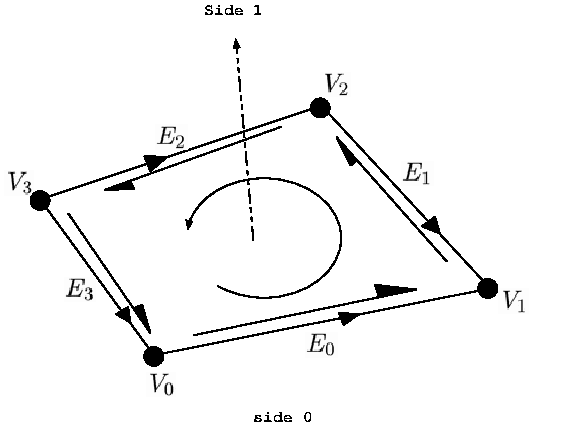
\includegraphics[scale=1.0]{figures/face_def} 
  \caption{Face definition}
  \label{fig:face_def}
  \end{center}
\end{figure}


\item[]{\bf {\em List\_ptr} MF\_Edges({\em MFace\_ptr} mface,
    {\em int} dir, {\em MVertex\_ptr} mvert):} Return the
  ordered set of edges of the face. The edges are ordered in the ccw
  while looking down the face 'normal' if dir is 1 and in the cw if
  dir is 0. If 'mvert' is specified, the edge set is reordered so that
  the first edge in the set contains this vertex. More precisely, if
  'dir' is 1, and the first edge is 'e' used in the face in direction
  'd', then {\bf ME\_Vertex(e,!d)} = mvert. With reference to
  Figure~\ref{fig:face_def}, the edges of the face in the ccw direction or
  'dir' = 1 are ${E_0,E_1,E_2,E_3}$ and in the opposite dir are
  ${E_3,E_2,E_1,E_0}$. If 'mvert' or the starting vertex is specified
  as $V_2$, the edge set in ccw direction or 'dir' = 1 is
  ${E_2,E_3,E_0,E_1}$ and in the opposite direction is
  ${E_1,E_0,E_3,E_2}$.  {\bf The list returned by this
  operator must be deleted by the calling application using {\em List\_Delete}}.

\item[]{\bf {\em List\_ptr} MF\_AdjFaces({\em MFace\_ptr} mface):}
List of adacent faces of a face. This operator is relevant only in
planar or surface surface meshes, i.e., for boundary faces not
connected to any regions.  {\bf The list returned by this
  operator must be deleted by the calling application using {\em List\_Delete}}.

\item[]{\bf {\em int} MF\_EdgeDir({\em MFace\_ptr} mface,
{\em MEdge\_ptr} medge):} Returns the direction in which the face
uses the given edge. If the faces use the edge in the positive direction,
the function returns 1; otherwise it returns 0.

\item[]{\bf {\em int} MF\_EdgeDir\_i({\em MFace\_ptr} mface,
{\em int} i):} Returns the direction in which the face uses its i'th
edge. If the face uses the edge in the positive direction the function
returns 1; otherwise it returns 0;

\item[]{\bf {\em List\_ptr} MF\_Regions({\em MFace\_ptr} mface):}
Return the set of regions connected to the face. If the face is not
used by any regions, the function returns NULL to indicate that the
set is empty. If not the set may contain one or two regions.  {\bf The list returned by this
  operator must be deleted by the calling application using {\em List\_Delete}}.

\item[]{\bf {\em MRegion\_ptr} MF\_Region({\em MFace\_ptr} mface,
{\em int} side):} Returns the region on the specified side of the
face. The positive side of the face (side = 1) is the side towards
which the face normal points. The negative side of the face (side = 0)
is the opposite side.

\item[]

\item[]{\bf {\em int} MF\_UsesEntity({\em MFace\_ptr} mface,
{\em MEntity\_ptr} mentity, {\em int} type):} Check if the face
uses the given lower dimension entity, 'mentity'. The type of the
entity is specified by the 'etype' variable. For a face, a lower
dimensional entity can be a vertex or an edge. If the face uses the
vertex or the edge, the function returns 1; otherwise it returns 0. If
any other type of entity is specified, the function returns 0.

\item[]{\bf {\em MFace\_ptr} MVs\_CommonFace({\em int} nv,
    {\em MVertex\_ptr} *fverts):} Return a face connected to all
  the given mesh vertices. Returns NULL if no such face exists.

\item[]{\bf {\em MFace\_ptr} MEs\_CommonFace({\em int} ne,
    {\em MEdge\_ptr} *fedges):} Return a face connected to all
  the given mesh edges. Returns NULL if no such face exists.

\item[]{\bf {\em int} MFs\_AreSame({\em MFace\_ptr} f1, {\em
      MFace\_ptr} f2):} {\em Applicable only to reduced
    representations}. Check if two faces described by vertices are
  equivalent. For example, a face described by vertices $\{1,2,3\}$ is
  equivalent to faces described by vertices $\{1,3,2\}$ and
  $\{3,1,2\}$.

\item[]

\item[]  {\bf {\em PType} MF\_PType({\em MFace\_ptr} v)}: Parallel entity type for face - can be PINTERIOR, POVERLAP or PGHOST.
\item[]  {\bf {\em int}   MF\_MasterParID({\em MFace\_ptr} v)}:
\item[]  {\bf {\em int}   MF\_GlobalID({\em MFace\_ptr} v)}:

\item[]
\item[]  The following three functions affect how mesh entities communicate and how their attributes are updated. IF YOU DON'T KNOW WHAT YOU ARE DOING WHEN YOU CALL THIS FUNCTION, YOU WILL GET WHAT YOU DESERVE.
\item[]  {\bf {\em void}  MF\_Set\_PType({\em MFace\_ptr} v, {\em PType} ptype)}: 
\item[]  {\bf {\em void}  MF\_Set\_MasterParID({\em MFace\_ptr} v, {\em int} masterparid)}
\item[]  {\bf {\em void}  MF\_Set\_GlobalID({\em MFace\_ptr} v, {\em int} globalid)}:  

\item[]

\item[]{\bf {\em void} MF\_Coords({\em MFace\_ptr} mface,
{\em int} *n, double (*xyz)[3], {\em int} dir):} Returns the
coordinates of the face vertices in an array along with the number of
vertices. 
% If 'dir' is 1, the coordinates are returned with a  ccw
% ordering while looking down the face normal; if 'dir' is 0, they are
% returned with a cw ordering (See Figure~\ref{fig:face_def}).

\item[]

\item[]{\bf {\em void} MF\_Lock({\em MFace\_ptr} f):} Lock a volatile
  face so that it cannot be deleted by garbage cleaning procedures (It
  can still be deleted by {\bf MF\_Delete}.

\item[]{\bf {\em void} MF\_UnLock({\em MFace\_ptr} f):} Unlock a volatile
  face so that it may be deleted freely by garbage cleaning procedures.


\end{description}

\newpage
\subsection{Mesh Region Object}

\begin{description}
\item[]{\bf {\em MRegion\_ptr} MR\_New({\em Mesh\_ptr}
    mesh):} Create a new region object. No topological information is
  embedded in the region when it is created. The region only knows
  which mesh it belongs to. The ID of the region is set by this
  function.

\item[]{\bf {\em void} MR\_Delete({\em MRegion\_ptr} mregion,
    {\em int} keep):} Delete the region. Deletes all topological
  information embedded in the region. If {\bf keep} is 0, the
  region is removed from the mesh and all topological and geometric
  information embedded in the region is destroyed. If {\bf keep} is
  1, the region is marked as type {\em MDELREGION} and removed from
  the mesh but the region is not destroyed. Also, the vertices, edges
  and faces of this region no longer point up to this region.
    
\item[]{\bf {\em void} MR\_Restore({\em MRegion\_ptr}
    mregion):} Restore a temporarily deleted region. The region type
  is restored from {\em MDELREGION} to {\em MREGION} and the
  region is added back to the mesh. The vertices, edges and faces of
  the region once again point back to the region.

\item[]
  
\item[]{\bf {\em void} MR\_Set\_GEntity({\em MRegion\_ptr}
    mregion, GEntity\_ptr gent):} Set the geometric model entity on
  which the region is classified.
  
\item[]{\bf {\em void} MR\_Set\_GEntDim({\em MRegion\_ptr}
    mregion, {\em int} gdim):} Set the dimension of the geometric
  model entity on which the region is classified.
  
\item[]{\bf {\em void} MR\_Set\_GEntID({\em MRegion\_ptr}
    mregion, {\em int} gid):} Set the ID of the geometric model
  entity on which the region is classified.
  
\item[]{\bf {\em void} MR\_Set\_GInfo\_Auto({\em MRegion\_ptr} mregion):}
  Derive the classification (GEntDim, GEntID) of the mesh region
  automatically (if possible) from the classification of its
  vertices or faces. If it is not possible to unambiguously get this
  information, the procedure will keep the default information. {\bf THIS
  MAY GET WRONG OR INCORRECT INFORMATION WHEN THERE IS AMBIGUOUS
  DATA.}


\item[]{\bf {\em void} MR\_Set\_ID({\em MRegion\_ptr}
    mregion, {\em int} id):} Explicitly set ID of a region and
  overwrite the ID set by the {\bf MR\_New} function. Does not
  check for duplication of region IDs.
  
\item[]{\bf {\em void} MR\_Set\_Faces({\em MRegion\_ptr}
    mregion, {\em int} nf, {\em MFace\_ptr} *mfaces,
    {\em int} *dirs):} Set the faces of the region along with their
  directions. The {\em unordered} set of faces and their directions
  are passed in through arrays along with the number of faces. If the
  normal of the face points out of the region, the associated
  direction to be passed in is 1; otherwise it is 0. This function is
  only relevant for full representations in MSTK.
  
\item[]{\bf {\em void} MR\_Set\_Vertices({\em MRegion\_ptr}
    mregion, {\em int} nv, {\em MVertex\_ptr} *mvertices, 
    {\em int} nf, {\em int} **rfv\_template):} Set
  the vertices of the region. This routine will collect/build all
  lower order topological information (edges, edge directions in the
  face) as needed by the face. For standard elements, the vertices
  must be ordered as indicated in Appendix~\ref{app:reg_conventions},
  while {\bf nf} can be 0 and {\bf rfv\_template} can be NULL.
  For non-standard elements, {\bf nf} is the number of faces of the
  polyhedron and {\bf rfv\_template} gives the vertices used in each
  face. More precisely, {\bf rfv\_template} has {\bf nfv}
  pointers to integer array $i$. The first entry of each
  {\bf rfv\_template$[i]$} represents the number of vertices in that
  face and the remaining entries represent the list of vertices of the
  face listed so that the face defined by them points out of the region.
  
\item[]{\bf {\em void} MR\_Replace\_Face({\em MRegion\_ptr}
    mregion, {\em MFace\_ptr} mface, {\em MFace\_ptr} nuface,
    {\em int} dir):} Replace a face of the region with another
  face. The direction in which the new face is used in the region must
  also be supplied. This function is only relevant for full
  representations in MSTK.
  
\item[]{\bf {\em void} MR\_Replace\_Vertex({\em MRegion\_ptr}
    mregion, {\em MVertex\_ptr} mvertex, {\em MVertex\_ptr}
    nuvertex):} Replace a vertex of a region with another vertex. This
  function is relevant only for reduced representations in MSTK.
  
\item[]{\bf {\em void}
    MR\_Replace\_Face\_i({\em MRegion\_ptr} mregion, {\em int}
    i, {\em MFace\_ptr} mface, {\em int} dir):} Replace the i'th
  face in the region with another face.The direction in which the new
  face is used in the region must also be supplied. This function is
  only relevant for full representations in MSTK.
  
\item[]{\bf {\em void}
    MR\_Replace\_Vertex\_i({\em MRegion\_ptr} mregion, {\em int}
    i, {\em MVertex\_ptr} mvertex):} Replace the i'th vertex of the
  region with another vertex. This function is only relevant for
  reduced representations in MSTK.

\item[]

  
\item[]{\bf {\em Mesh\_ptr} MR\_Mesh({\em MRegion\_ptr}
    mregion):} Returns the mesh that the region belongs to.
  
\item[]{\bf {\em int} MR\_ID({\em MRegion\_ptr} mregion):}
  Returns the ID of the region. Returns 0 if not known.
  
\item[]{\bf {\em int} MR\_GEntDim({\em MRegion\_ptr}
    mregion):} Returns the dimension of the geometric model entity the
  region is classified on. Always returns 3 since a mesh region can be
  classified only on a model region.
  
\item[]{\bf {\em int} MR\_GEntID({\em MRegion\_ptr}
    mregion):} Returns the ID of the geometric model entity that the
  region is classified on. Returns 0 if not known.
  
\item[]{\bf {\em GEntity\_ptr} MR\_GEntity({\em MRegion\_ptr}
    mregion):} Returns a pointer or handle to the geometric model
  entity that the vertex is classified on. Returns NULL if this
  information is not known.

\item[]

\item[]{\bf {\em int} MR\_Num\_Vertices({\em MRegion\_ptr}
mregion):} Returns the number of vertices of a region.

\item[]{\bf {\em int} MR\_Num\_Edges({\em MRegion\_ptr} mregion):}
Returns the number of edges of a region.

\item[]{\bf {\em int} MR\_Num\_Faces({\em MRegion\_ptr} mregion):}
Returns the number of faces of a region.

\item[]{\bf {\em int} MR\_Num\_AdjRegions({\em MRegion\_ptr}
mregion):} Returns the number of adjacent regions of a region, i.e.,
regions sharing a face with this region.

\item[] 

\item[]{\bf {\em List\_ptr} MR\_Vertices({\em MRegion\_ptr}
mregion):} Returns the set of vertices of a region. For standard
elements the vertices are ordered as indicated in
Appendix~\ref{app:reg_conventions}. For non-standard elements the set
is unordered. {\bf The list returned by this
  operator must be deleted by the calling application using {\em List\_Delete}}.

\item[]{\bf {\em List\_ptr} MR\_Edges({\em MRegion\_ptr} mregion):}
Return the \underline{unordered} set of edges of a region.  {\bf The list returned by this
  operator must be deleted by the calling application using {\em List\_Delete}}.

\item[]{\bf {\em List\_ptr} MR\_Faces({\em MRegion\_ptr} mregion):}
Returns the set of faces of a region. {\bf The list returned by this
  operator must be deleted by the calling application using {\em List\_Delete}}.

\item[]{\bf {\em List\_ptr} MR\_AdjRegions({\em MRegion\_ptr}
mregion):} Returns the set of adjacent regions of a region, i.e.,
regions sharing a face with this region. The set is not ordered.

\item[]{\bf {\em int} MR\_FaceDir({\em MRegion\_ptr} mregion,
{\em MFace\_ptr} mface):} Returns the direction in which the region
uses the given face. Returns 1 if the face normal points out of the
region and returns 0 if the face normal points into the region.

\item[]{\bf {\em int} MR\_FaceDir\_i({\em MRegion\_ptr} mregion,
{\em int} i):} Returns the direction in which the region uses the
i'th face. Returns 1 if the face normal points out of the region and
returns 0 if the face normal points into the region.


\item[]

\item[]{\bf {\em int} MR\_UsesEntity({\em MRegion\_ptr} mregion,
{\em MEntity\_ptr} ment, {\em int} type):} Check if the region
uses the given lower dimension entity, 'mentity'. The type of the
entity is

\item[]

\item[]  {\bf {\em PType} MR\_PType({\em MRegion\_ptr} v)}: Parallel entity type for edge - can be PINTERIOR, POVERLAP or PGHOST.
\item[]  {\bf {\em int}   MR\_MasterParID({\em MRegion\_ptr} v)}:
\item[]  {\bf {\em int}   MR\_GlobalID({\em MRegion\_ptr} v)}:

\item[]
\item[]  The following three functions affect how mesh entities communicate and how their attributes are updated. IF YOU DON'T KNOW WHAT YOU ARE DOING WHEN YOU CALL THIS FUNCTION, YOU WILL GET WHAT YOU DESERVE.
\item[]  {\bf {\em void}  MR\_Set\_PType({\em MRegion\_ptr} v, {\em PType} ptype)}: 
\item[]  {\bf {\em void}  MR\_Set\_MasterParID({\em MRegion\_ptr} v, {\em int} masterparid)}
\item[]  {\bf {\em void}  MR\_Set\_GlobalID({\em MRegion\_ptr} v, {\em int} globalid)}:  

\item[]

\item[]{\bf {\em void} MR\_Coords({\em MRegion\_ptr} mregion,
{\em int} *n, double (*xyz)[3]):} Returns the coordinates of the
region vertices in an array along with the number of vertices. For
standard elements, the ordering is as given in
Appendix~\ref{app:reg_conventions}. For non-standard elements, the
ordering is arbitrary.
\end{description}



\newpage
\subsection{Generic Entity Object}

The following functions operate on generic mesh entities of type
{\em MEntity\_ptr}. This implies that variables of type
{\em MVertex\_ptr}, {\em MEdge\_ptr}, {\em MFace\_ptr},
{\em MRegion\_ptr} can all be passed in place of
{\em MEntity\_ptr} variables in the following functions.

\begin{description}
%%  {\em void} MEnt\_Set\_GEntity({\em MEntity\_ptr} mentity, GEntity\_ptr gent);
%%
%%  {\em void} MEnt\_Set\_GEntDim({\em MEntity\_ptr} mentity, {\em int} gdim);
%%
%%  {\em void} MEnt\_Set\_ID({\em MEntity\_ptr} mentity, {\em int} id);

  
\item[]{\bf {\em int} MEnt\_ID({\em MEntity\_ptr} mentity):} Returns
the ID of a generic entity.

\item[]{\bf {\em int} MEnt\_Dim({\em MEntity\_ptr} mentity):}
Returns the topological dimension or type of generic entity.

\item[]{\bf {\em int} MEnt\_OrigDim({\em MEntity\_ptr} mentity):}
Returns the original topological dimension or type of generic entity before it
was temporarily deleted.

\item[]{\bf {\em int} MEnt\_IsVolatile({\em MEntity\_ptr}) mentity):}
  Is the entity a temporary (volatile) entity in a reduced
  representation or an explicitly represented persistent entity. For
  example, this query will return 1 on any edge in a reduced
  representation.

\item[]{\bf {\em Mesh\_ptr} MEnt\_Mesh({\em MEntity\_ptr} mentity):}
Returns the mesh that the entity belongs to.

\item[]{\bf {\em int} MEnt\_GEntDim({\em MEntity\_ptr}
    mentity):} Returns the dimension of the geometric model entity
  that the entity is classified on.
  
\item[]{\bf {\em GEntity\_ptr}
    MEnt\_GEntity({\em MEntity\_ptr} mentity):} Returns a pointer
  or handle to geometric model entity that the entity is classified
  on.

\item[]{\bf {\em void} MEnt\_Delete({\em MEntity\_ptr} mentity, {\em
      int} keep):} Delete a generic mesh entity. If {\bf keep} is 0,
  the entity is removed from the mesh and all topological and
  geometric information embedded in the entity is destroyed. If {\bf
    keep} is 1, the region is marked as deleted and removed from the
  mesh but the entity is not destroyed. Also, lower order entities in
  the mesh no longer point up to this entity.

\item[]
  
\item[]{\bf {\em void} MEnt\_Set\_AttVal({\em MEntity\_ptr} ent, {\em
      MAttrib\_ptr} attrib, {\em int} ival, {\em double} lval, {\em
      void} *pval):} Set the value of an attribute for given mesh
  entity. Depending on the attribute type, different arguments of this
  function are relevant. If the attribute type is:

\begin{itemize}
  \item {\bf INT} -- specify the integer value in {\bf ival},
  \item {\bf DOUBLE} -- specify the the real value in {\bf rval},
  \item {\bf VECTOR} -- specify a pointer to an array of
    doubles in {\bf pval}\footnote{Remember to not free the array specified in {\bf pval} without telling the attribute system because MSTK stores the pointer to the array directly and does not make a copy of the array.} - the number of doubles should equal the number components specified in the definition of the VECTOR attribute,
  \item {\bf TENSOR} -- specify a pointer
    to an array of doubles in {\bf pval} - the number of doubles should equal the number of components specified in the definition of the TENSOR attribute,
  \item {\bf POINTER} -- specify the pointer value in {\bf pval}.
  \end{itemize}


    
\item[]{\bf {\em void} MEnt\_Rem\_AttVal({\em MEntity\_ptr}
    ent, {\em MAttrib\_ptr mattrib}:} Clear the value of the given
  attribute from the entity.
    
\item[]{\bf {\em int} MEnt\_Get\_AttVal({\em MEntity\_ptr} ent, {\em
      MAttrib\_ptr} int *ival, double *rval, double **pval):} Get the
  value of an attribute from an entity.  Depending on the attribute
  type, different arguments of this function are relevant. If the
  attribute type is:

  \begin{itemize}
  \item {\bf INT} -- {\bf ival} contains the integer value,
  \item {\bf DOUBLE} -- {\bf rval} contains the real value,
  \item {\bf VECTOR} -- {\bf pval} contains a pointer to an array of doubles,
  \item {\bf TENSOR} -- {\bf pval} contains a pointer
    to an array of doubles,
  \item {\bf POINTER} -- {\bf pval} conntains the pointer value.
  \end{itemize}

\item[]{\bf {\em void} MEnt\_Rem\_AllAttVals({\em MEntity\_ptr}):}
  Remove all attribute values attached to an entity.

\end{description}

\newpage
\subsection{Mesh Attributes}

\begin{description}
  
\item[]{\bf {\em MAttrib\_ptr} MAttrib\_New({\em Mesh\_ptr} mesh, {\em
      const char} *att\_name, {\em MAttType} att\_type, {\em MType}
    entdim, $<${\em int ncomponents}$>$):} Define a new mesh
  attribute. Along with the mesh to which this attribute is assigned
  ({\bf mesh}) and the name of the attribute ({\bf att\_name}), the
  type of the attribute ({\bf att\_type}) must be specified as {\bf
    INT}, {\bf DOUBLE}, {\bf VECTOR}, {\bf TENSOR} or {\bf
    POINTER}. Also, the dimension of the entity for which the
  attribute value can be set must be specified as {\bf MVERTEX}, {\bf
    MEDGE}, {\bf MFACE}, {\bf MREGION} or {\bf MALLTYPE}. The last
  argument {\em {\bf ncomponents}} is an optional argument for attributes of
  type {\bf INT}, {\bf DOUBLE} or {\bf POINTER} but is required for
  attributes of type {\bf VECTOR} and {\bf TENSOR}.

\item[]{\bf {\em char} *MAttrib\_Get\_Name({\em MAttrib\_ptr}
    attrib, {\em char} *att\_name):} Get the name of the given attribute.
  
\item[]{\bf {\em MAttType}
    MAttrib\_Get\_Type({\em MAttrib\_ptr} attrib):} Get the type of
  the attribute (Can return {\bf INT}, {\bf DOUBLE},
  {\bf PVAL}).
  
\item[]{\bf {\em MType}
    MAttrib\_Get\_EntDim({\em MAttrib\_ptr} attrib):} Get the
  dimension (or type) of entity attribute can be asssigned to. Can be
  {\bf MVERTEX}, {\bf MEDGE}, {\bf MFACE}, {\bf MREGION}
  or {\bf MALLTYPE}.
  
\item[]{\bf {\em void} MAttrib\_Delete({\em MAttrib\_ptr}
    attrib):} Delete an attribute.

\end{description}

\newpage
\subsection{Mesh Sets}

Mesh sets are unordered but named sets of entities. MSets can be
queried and modified just like Lists. However, unlike Lists, MSets are
associated with a mesh, can be constrained to contain only particular
types of entities and have boolean operations performed on them.

\begin{description}
  
\item[]{\bf {\em MSet\_ptr} MSet\_New({\em Mesh\_ptr} mesh, {\em const
      char} *set\_name, {\em MType} entdim):} Define a new mesh entity
  set. Along with the mesh to which this set is assigned ({\bf mesh})
  and the name of the set ({\bf att\_name}), the the dimension of the
  entities that the set can contain must be specified as {\bf
    MVERTEX}, {\bf MEDGE}, {\bf MFACE}, {\bf MREGION} or {\bf
    MALLTYPE}.

\item[]{\bf {\em char} *MSet\_Name({\em MSet\_ptr} set, {\em char}
    *att\_name):} Get the name of the given set.
  
\item[]{\bf {\em MType} MSet\_EntDim({\em MSet\_ptr} set):} Get the
  dimension of entities the set can contain. Can be {\bf MVERTEX},
  {\bf MEDGE}, {\bf MFACE}, {\bf MREGION} or {\bf MALLTYPE}.
  
\item[]{\bf {\em Mesh\_ptr} MSet\_Mesh({\em MSet\_ptr} set):}
Returns the mesh that the entity set belongs to.

\item[]{\bf {\em void} MSet\_Delete({\em MSet\_ptr} set):} Delete an
  set.

\item[]{\bf {\em MSet\_ptr} MSet\_Add({\em MSet\_ptr} l, {\em void
      *}entry):} Add an entry to the set. The entry is strictly
  appended to the end of the set.

\item[]{\bf {\em MSet\_ptr} MSet\_ChknAdd({\em MSet\_ptr} l, {\em void
      *}entry):} Add an entry to a set only if it is not already in
  the set.

\item[]{\bf {\em MSet\_ptr} MSet\_Insert({\em MSet\_ptr} l, {\em void
      *}nuentry, {\em void *}b4entry):} Insert an entry into the set
  in the position before 'b4entry'.

\item[]{\bf {\em MSet\_ptr} MSet\_Inserti({\em MSet\_ptr} l, {\em void
      *}nuentry, {\em int} i):} Insert an entry into the set at the
  i'th valid position and push the entries previously at the i'th and
  later position back.

\item[]{\bf {\em int} MSet\_Rem({\em MSet\_ptr} l, {\em void
      *}entry):} Remove an entry from the set. Returns 1 if
  successful, 0 otherwise.

\item[]{\bf {\em int} MSet\_Remi({\em MSet\_ptr} l, {\em int} i):}
  Remove the i'th valid entry in the set. Returns 1 if successful, 0
  otherwise.

\item[]{\bf {\em int} MSet\_Replace({\em MSet\_ptr} l, {\em void
      *}entry, {\em void *}nuentry):} Replace 'entry' with 'nuentry'
  in set. Returns 1 if successful, 0 otherwise.

\item[]{\bf {\em int} MSet\_Replacei({\em MSet\_ptr} l, {\em int} i,
    void *nuentry):} Replace the i'th valid entry in the set with
  'nuentry'. Returns 1 if successful, 0 otherwise.

\item[]{\bf {\em int} MSet\_Contains({\em MSet\_ptr} l, void *entry):}
  Returns 1 if set contains the entry, 0 otherwise.

\item[]{\bf {\em int} MSet\_Locate({\em MSet\_ptr} l, void *entry):}
  Returns the positional index of the entry in the set. Returns -1 if
  the set does not contain the entry.

\item[]{\bf {\em void *}MSet\_Entry({\em MSet\_ptr} l, {\em int} i):}
  Return the i'th valid entry in the set.  Returns a NULL pointer if
  the i'th valid entry could not be found.

\item[]{\bf {\em void *}MSet\_Next\_Entry({\em MSet\_ptr} l, {\em int}
    *i):} Return the next valid entry in the set. This routine works
  just like List\_Next\_Entry.

\item[]{\bf {\em int} MSet\_Num\_Entries({\em MSet\_ptr} l):} Return
  the number of entries in a set.

\item[]{\bf {\em MSet\_ptr} MSets\_Union({\em MSet\_ptr} s1, {\em
      MSet\_ptr} s2):} Create a new set from the union of two sets.

\item[]{\bf {\em MSet\_ptr} MSets\_Intersect({\em MSet\_ptr} s1, {\em
      MSet\_ptr} s2):} Create a new set from the intersection of two
  sets. Routine returns null if the intersection is a null set.

\item[]{\bf {\em MSet\_ptr} MSets\_Subtract({\em MSet\_ptr} s1, {\em
      MSet\_ptr} s2):} Create a new set by subtracting set 2 from set
  1. Routine returns null if the result is a null set.

\end{description}

\newpage
\subsection{Entity Marks}

Entity marks or markers are a way of tagging entities. Such
functionality is useful in algorithms which must keep track of
processed entities to avoid duplication of work. An example of such an
operation is creating a union of entity sets while extracting upward
adjacency information such as the regions connected to an edge. Use of
entity marks avoids calling {\bf List\_ChknAdd} (search through the
list and add item if it is not there) or using attributes to tag
entities with 0 or 1. As a result it is much more efficient than
either option.

\begin{description}
\item[]{\bf {\em int} MSTK\_GetMarker():} Returns a unique marker ID
which may be used to tag entities.

\item[]{\bf {\em void} MEnt\_Mark({\em MEntity\_ptr} ent, {\em int} mkr):} Mark an entity with the given marker 'mkr'.

\item[]{\bf {\em int} MEnt\_IsMarked({\em MEntity\_ptr} ent, {\em int} mkr):} Check if an entity is marked with the given marker 'mkr'.

\item[]{\bf {\em void} MEnt\_Unmark({\em MEntity\_ptr} ent, {\em int} mkr):} Unmark an entity with respect to the given marker 'mkr'

\item[]{\bf {\em void} List\_Mark({\em List\_ptr} list, {\em int} mkr):} Mark a list of entities with given marker.

\item[]{\bf {\em void} List\_Unmark({\em List\_ptr} list, {\em int} mkr):}
Unmark a list of entities with respect to the given marker.

\item[]{\bf {\em void} MSet\_Mark({\em MSet\_ptr} list, {\em int} mkr):} Mark a set of entities with given marker.

\item[]{\bf {\em void} MSet\_Unmark({\em MSet\_ptr} list, {\em int} mkr):}
Unmark a set of entities with respect to the given marker.

\item[]{\bf {\em void} MSTK\_FreeMarker({\em int} mkr):} Release the
marker ID given by {\bf MSTK\_GetMarker()} so that it can be
reused. Care must be taken to unmark all entities marked with this
marker ID before releasing it. If not, subsequent operations with
reassigned marker will find a tag on some entities and mistake them
for being processed.
\end{description}

An example use of entity marks is given below:

\newpage
\begin{verbatim}

/* Code to get the faces of a vertex */
/* NOTE: This code is for illustration of entity marks only. */
/*       This functionality is already available through MV_Faces */

vedges = MV_Edges(v);      /* Edges of vertex */

mkid = MSTK_GetMarker();   /* Get a new marker */
vfaces = List_New(10);     /* Initialize list of faces cncted to v */

idx = 0;
while ((ve = List_Next_Entry(vedges,&idx))) {   /* For each edge */

  efaces = ME_Faces(ve);                /* Get faces of edge */
  idx1 = 0;
  while ((ef = List_Next_Entry(efaces,&idx1))) {
    if (!MEnt_IsMarked(ef,mkid)) {         /* Is the face already in list? */
      List_Add(vfaces,ef);                 /* No? Add it to the list and   */
      MEnt_Mark(ef,mkid);                  /* mark it as being in the list */
    }
  }
  List_Delete(efaces);

}

List_Delete(vedges);

List_Unmark(vfaces,mkid);                 /* Unmark all the marked faces */
MSTK_FreeMarker(mkid);                    /* Very important to free the marker!! */
                                          /* otherwise, we'll run out of markers */
\end{verbatim}


\newpage 
\subsection{Parallel Mesh Management}

The following are the highest level of parallel mesh management functions.

\begin{description}

\item[] {\bf {\em int} MSTK\_Mesh\_Read\_Distribute({\em Mesh\_ptr
      *}recv\_mesh, {\em const char*} global\_mesh\_name, {\em int} *dim,
    {\em int} ring, {\em int} with\_attr, {\em int} rank, {\em int}
    num, {\em MPI\_Comm} comm)}: Routine reads a mesh of dimension
  'dim' from file 'global\_mesh\_name' on processor 'rank' and
  distributes it 'num' processors. 'comm' is the communicator to be
  used by MPI. If 'ring' is 0, there is no overlap of the highest
  level entities between processors - only entities on processor
  boundaries will be duplicated on other processors. If 'ring' is N,
  then 'N' layers of the highest level entities will overlap between
  processors ({\em Currently, only 1 layer of overlap elements are
    supported}). If 'with\_attr' is 1, then MSTK sets up the links
  necessary to synchronize attribute data across processors. This routine must be called from only one processor.

\item[] {\bf {\em int} MSTK\_Mesh\_Distribute({\em Mesh\_ptr
      *}recv\_mesh, {\em int} *dim, {\em int} ring, {\em int}
    with\_attr, {\em int} rank, {\em int} num, {\em MPI\_Comm} comm)}:
  Similar to the above Read\_Distribute routine except that it does
  not do any read. On the root processor, 'recv\_mesh' is an
  input-output parameter - the application uses it to send in the full
  mesh to be distributed and the mesh partition belonging to the root
  processor is returned in it. On other processors, this is an output
  parameter only. Also, 'dim', indicating the topological dimension of
  the input mesh, is an input parameter on the root processor while it
  is an output parameter on the other processors.


\item[] {\bf {\em int} MSTK\_UpdateAttr({\em Mesh\_ptr} mesh, {\em
      int} rank, {\em int} num, {\em MPI\_Comm} comm)}: Update the
  attributes of duplicated entities on remote processors.

\end{description}

For users requiring more fine grain control of their application, the
following a list of lower level parallel mesh functions. Descriptions
of these functions will be added soon. {\bf NOTE THAT THESE ROUTINES
  HAVE NOT IN ANYWAY BEEN MADE IDIOT-PROOF AND REQUIRE GOOD KNOWLEDGE
  OF THE PARALLEL MODEL IN MSTK.}

\begin{description}

  \item[] {\bf {\em int} MSTK\_SendMesh({\em Mesh\_ptr} mesh, {\em int} rank, {\em int} with\_attr, {\em MPI\_Comm} comm)}:

  \item[] {\bf {\em int} MSTK\_RecvMesh({\em Mesh\_ptr} mesh, {\em int} dim, {\em int} send\_rank, {\em int} rank, {\em int} with\_attr, {\em MPI\_Comm} comm)}:


  \item[] {\bf {\em int} MESH\_PartitionWithMetis({\em Mesh\_ptr} mesh, {\em int} nparts, {\em int} **part)}:
  \item[] {\bf {\em int}        MSTK\_Mesh\_Partition({\em Mesh\_ptr} mesh, {\em Mesh\_ptr} *submeshes, {\em int} num, 				 {\em int} ring, {\em int} with\_attr)}
  \item[] {\bf {\em int}        MESH\_Partition({\em Mesh\_ptr} mesh, {\em Mesh\_ptr} *submeshes, {\em int} num)}
  \item[] {\bf {\em int}        MESH\_CopyAttr({\em Mesh\_ptr} mesh, {\em Mesh\_ptr} submesh, {\em const char} *attr\_name)}


  \item[] {\bf {\em int}        MESH\_BuildPBoundary({\em Mesh\_ptr} mesh, {\em Mesh\_ptr} submesh)}


  \item[] {\bf {\em int}        MESH\_AddGhost({\em Mesh\_ptr} mesh, {\em Mesh\_ptr} submesh, {\em int} part\_no, {\em int} ring)}

  \item[] {\bf {\em int}        MESH\_SendMesh({\em Mesh\_ptr} mesh, {\em int} rank, {\em MPI\_Comm} comm)}
  \item[] {\bf {\em int}        MESH\_SendAttr({\em Mesh\_ptr} mesh, {\em const char} *attr\_name, {\em int} rank, {\em MPI\_Comm} comm)}
  \item[] {\bf {\em int}        MESH\_RecvMesh({\em Mesh\_ptr} mesh, {\em int} dim, {\em int} send\_rank, {\em int} rank, {\em MPI\_Comm} comm)}
  \item[] {\bf {\em int}        MESH\_RecvAttr({\em Mesh\_ptr} mesh, {\em const char} *attr\_name, {\em int} rank, {\em int} recv\_rank, {\em MPI\_Comm} comm)}


  \item[]{\bf {\em int} MESH\_Num\_GhostVertices({\em Mesh\_ptr} mesh):}
    Number of ghost vertices in the mesh.

  \item[]{\bf {\em int} MESH\_Num\_GhostEdges({\em Mesh\_ptr} mesh):}
    Number of ghost edges in the mesh.

  \item[]{\bf {\em int} MESH\_Num\_GhostFaces({\em Mesh\_ptr} mesh):}
    Number of ghost faces in the mesh. 

  \item[]{\bf {\em int} MESH\_Num\_GhostRegions({\em Mesh\_ptr} mesh):}
    Number of ghost regions in the mesh.

  \item[]

  \item[]{\bf {\em MVertex\_ptr} MESH\_GhostVertex({\em Mesh\_ptr} mesh,
      {\em int} i):} Return the i'th ghost vertex in the mesh. Returns NULL if i
    $<$ 0 or i $>$ number of mesh vertices.

  \item[]{\bf {\em MEdge\_ptr} MESH\_GhostEdge({\em Mesh\_ptr} mesh,
      {\em int} i):} Return the i'th ghost edge in the mesh. Returns NULL if i $<$
    0 or i $>$ number of mesh edges. Returns NULL for reduced
    representations.

  \item[]{\bf {\em MFace\_ptr} MESH\_GhostFace({\em Mesh\_ptr} mesh,
      {\em int} i):} Return the i'th face in the mesh. Returns NULL if i $<$
    0 or i $>$ number of mesh faces. Only faces explicitly represented in
    the mesh are returned for reduced representation.

  \item[]{\bf {\em MRegion\_ptr} MESH\_GhostRegion({\em Mesh\_ptr} mesh, {\em
        int} i):} Return the i'th region in the mesh. Returns NULL if i
    $<$ 0 or i $>$ number of mesh region.

  \item[]

  \item[]{\bf {\em MVertex\_ptr} MESH\_Next\_GhostVertex({\em Mesh\_ptr}
      mesh, {\em int} *idx):} Returns the next ghost vertex while iterating
    through the vertices of the mesh. See the routine {\bf
      List\_Next\_Entry} above for an explanation of how the iteration
    works. This routine is in general faster than using the routine {\bf
      MESH\_GhostVertex}.

  \item[]{\bf {\em MEdge\_ptr} MESH\_Next\_GhostEdge({\em Mesh\_ptr} mesh,
      {\em int} *idx):} Returns the next ghost edge while iterating through the
    edges of the mesh. See the routine List\_Next\_Entry above for an
    explanation of how the iteration works.  The routine always returns
    NULL for reduced representations.

  \item[]{\bf {\em MFace\_ptr} MESH\_Next\_GhostFace({\em Mesh\_ptr} mesh,
      {\em int} *idx):} Returns the next ghost face while iterating through the
    faces of the mesh. See the routine {\bf List\_Next\_Entry} above for
    an explanation of how the iteration works.  Only faces explicitly
    represented in the mesh are returned for reduced representation.

  \item[]{\bf {\em MRegion\_ptr}
      MESH\_Next\_GhostRegion({\em Mesh\_ptr} mesh, {\em int} *idx):}
    Returns the next region while iterating through the regions of the
    mesh. See the routine {\bf List\_Next\_Entry} above for an
    explanation of how the iteration works.
    
  \item[]

  \item[]{\bf {\em int} MESH\_Num\_OverlapVertices({\em Mesh\_ptr} mesh):}
    Number of overlap vertices in the mesh.

  \item[]{\bf {\em int} MESH\_Num\_OverlapEdges({\em Mesh\_ptr} mesh):}
    Number of overlap edges in the mesh.

  \item[]{\bf {\em int} MESH\_Num\_OverlapFaces({\em Mesh\_ptr} mesh):}
    Number of overlap faces in the mesh. 

  \item[]{\bf {\em int} MESH\_Num\_OverlapRegions({\em Mesh\_ptr} mesh):}
    Number of overlap regions in the mesh.

  \item[]

  \item[]{\bf {\em MVertex\_ptr} MESH\_OverlapVertex({\em Mesh\_ptr} mesh,
      {\em int} i):} Return the i'th overlap vertex in the mesh. Returns NULL if i
    $<$ 0 or i $>$ number of mesh vertices.

  \item[]{\bf {\em MEdge\_ptr} MESH\_OverlapEdge({\em Mesh\_ptr} mesh,
      {\em int} i):} Return the i'th overlap edge in the mesh. Returns NULL if i $<$
    0 or i $>$ number of mesh edges. Returns NULL for reduced
    representations.

  \item[]{\bf {\em MFace\_ptr} MESH\_OverlapFace({\em Mesh\_ptr} mesh,
      {\em int} i):} Return the i'th face in the mesh. Returns NULL if i $<$
    0 or i $>$ number of mesh faces. Only faces explicitly represented in
    the mesh are returned for reduced representation.

  \item[]{\bf {\em MRegion\_ptr} MESH\_OverlapRegion({\em Mesh\_ptr} mesh, {\em
        int} i):} Return the i'th region in the mesh. Returns NULL if i
    $<$ 0 or i $>$ number of mesh region.

  \item[]

  \item[]{\bf {\em MVertex\_ptr} MESH\_Next\_OverlapVertex({\em Mesh\_ptr}
      mesh, {\em int} *idx):} Returns the next overlap vertex while iterating
    through the vertices of the mesh. See the routine {\bf
      List\_Next\_Entry} above for an explanation of how the iteration
    works. This routine is in general faster than using the routine {\bf
      MESH\_OverlapVertex}.

  \item[]{\bf {\em MEdge\_ptr} MESH\_Next\_OverlapEdge({\em Mesh\_ptr} mesh,
      {\em int} *idx):} Returns the next overlap edge while iterating through the
    edges of the mesh. See the routine List\_Next\_Entry above for an
    explanation of how the iteration works.  The routine always returns
    NULL for reduced representations.

  \item[]{\bf {\em MFace\_ptr} MESH\_Next\_OverlapFace({\em Mesh\_ptr} mesh,
      {\em int} *idx):} Returns the next overlap face while iterating through the
    faces of the mesh. See the routine {\bf List\_Next\_Entry} above for
    an explanation of how the iteration works.  Only faces explicitly
    represented in the mesh are returned for reduced representation.

  \item[]{\bf {\em MRegion\_ptr}
      MESH\_Next\_OverlapRegion({\em Mesh\_ptr} mesh, {\em int} *idx):}
    Returns the next region while iterating through the regions of the
    mesh. See the routine {\bf List\_Next\_Entry} above for an
    explanation of how the iteration works.
    
\end{description}



\newpage
\subsection{Mesh Modification}

\begin{description}

\item[]{\bf {\em int} ME\_Swap2D({\em MEdge\_ptr} e,
{\em MEdge\_ptr} *enew, {\em MFace\_ptr} fnew[2]):} Swap an edge
in a triangular mesh. No checks are performed for topological or
geometric validity.

\item[]{\bf {\em MVertex\_ptr} MVs\_Merge({\em MVertex\_ptr} v1, {\em
      MVertex\_ptr} v2):} Merge two vertices, v1 and v2, and return
  the retained vertex. By default, v1 is retained.

\item[]{\bf {\em MFace\_ptr} MFs\_Join({\em MFace\_ptr} f1,
{\em MFace\_ptr} f2, {\em MEdge\_ptr} e):} Join two faces along
common edge and create new face by eliminating the common edge as
shown in Figure~\ref{fig:MFs_Join}. If 'f1' has 'n1' edges and 'f2'
has 'n2' edges, then the new face has ('n1'+'n2'-2) edges.

\end{description}

\begin{figure}[!h]
  \begin{center}
    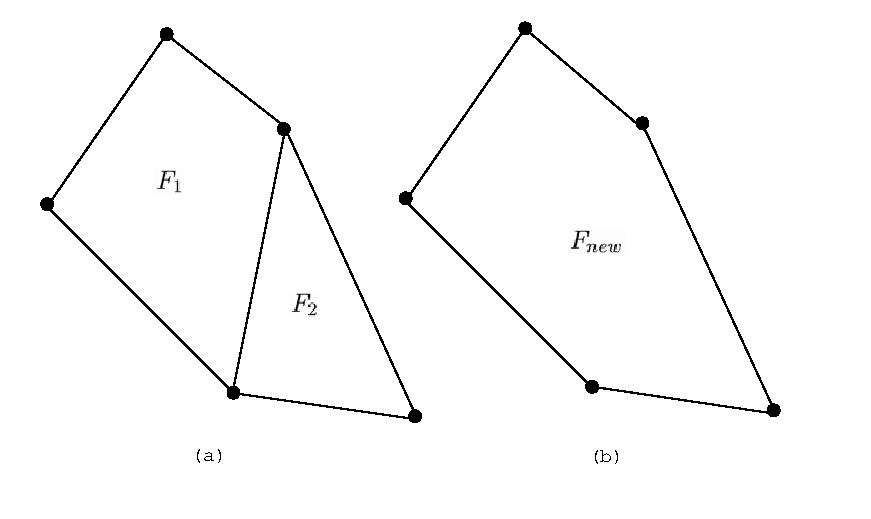
\includegraphics[scale=1.0]{figures/MFs_Join}
    
    \caption{Joining two faces (a) Two faces $F_1$ and $F_2$ sharing a
      common edge (b) New pentagonal face $F_{new}$ created by
      eliminating the common edge.  }
    \label{fig:MFs_Join}
  \end{center}
\end{figure}

\newpage
\subsection{Utilities}
  
\begin{description}
  
\item[]{\bf {\em void} MSTK\_Report({\em char} *module,
  {\em char} *message, {\em ErrType} severity):} Error handler
  for MSTK. 'module' is the name of the function in which the error
  occurs. 'message' is the error message and is recommended to be less
  than 1024 characters in length. 'severity' is an error code and can
  be MESSG, WARN, ERROR or FATAL. If the error code is FATAL, the
  program will quit after printing the error. If the same message is
  repeated successively, then the message is printed only the first
  time.

\item[]{\bf {\em void} List\_PrintID({\em List\_ptr} l):} Debugging
utility to print the IDs of the entities in a set.

\item[]{\bf {\em void} MV\_Print({\em MVertex\_ptr} v, int
    lev):} Debugging utility to print information about a mesh vertex,
  {\bf v}. The argument {\bf lev} controls the level of detail
  of the information printed. {\bf lev} = 0 prints the minimum
  information, i.e., vertex pointer, its ID and its coordinates. If
  {\bf lev} = 1, the function prints classification information for
  the vertex (if available), i.e., ID and dimension of the model
  entity that the vertex is on. If {\bf lev} $>$ 1, then upward
  detailed adjacency information is also printed for the vertex, i.e.,
  information is printed about the edges, faces and regions connected
  to the vertex.
  
\item[]{\bf {\em void} ME\_Print({\em MEdge\_ptr} e, int
    lev):} Debugging utility to print information about a mesh edge,
  {\bf e}. The argument {\bf lev} controls the level of detail
  of the information printed. {\bf lev} = 0 prints the minimum
  information, i.e., edge pointer, its ID and the IDs of its two
  vertices. If {\bf lev} = 1, the function prints classification
  information for the edge (if available), i.e., ID and dimension of
  the model entity that the edge is on. Also, more detailed vertex
  information printed in this case. If {\bf lev} $>$ 1, the
  function prints detailed upward adjacency information for the edge,
  i.e., information is printed about the faces and regions connected
  to the edge.
    
  \item[]{\bf {\em void} MF\_Print({\em MFace\_ptr} f, int
      lev):} Debugging utility to print information about a mesh face,
    {\bf f}. The argument {\bf lev} controls the level of detail
    of the information printed. {\bf lev} = 0 prints the minimum
    information, i.e., the face pointer and its ID. If {\bf lev} =
    1, the function prints classification information for the edge (if
    available), i.e., ID and dimension of the model entity that the
    face is on. Also, a signed list of the edges of the face is
    printed.  If {\bf lev} $>$ 1, the function prints detailed
    downward and upward adjacency information for the face, i.e.,
    information is printed about the edges and vertices of the face,
    and about the regions connected to the face.
    
  \item[]{\bf {\em void} MR\_Print({\em MRegion\_ptr} r, int
      lev):} Debugging utility to print information about a mesh
    region, {\bf r}. The argument {\bf lev} controls the level
    of detail of the information printed. {\bf lev} = 0 prints the
    minimum information, i.e., region pointer and its ID. If
    {\bf lev} = 1, the function prints classification information
    for the region (if available), i.e., ID of the model entity that
    the region is on. Also, a signed list of the faces of the region
    is printed. If {\bf lev} $>$ 1, the function prints detailed
    downward adjacency information for the region, i.e., information
    is printed about the faces, edges and vertices forming the region.



\end{description}

\newpage
\appendix

\section{Conventions for Vertex, Edge Numbering in Standard Region Types}
\label{app:reg_conventions}

\begin{figure}[!h]
  \begin{center}
    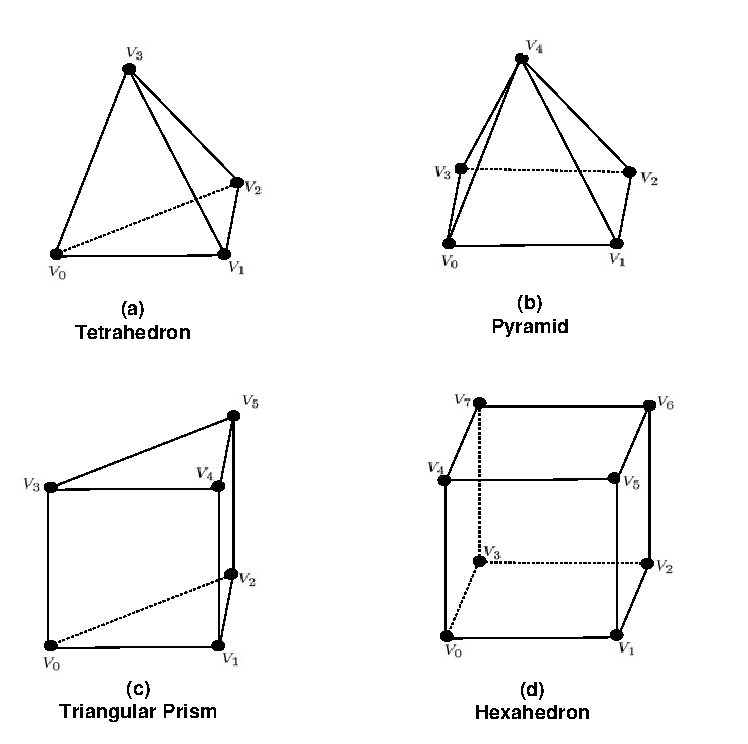
\includegraphics[scale=1.0]{figures/reg_conventions}
  \end{center}
\end{figure}

\newpage
\section{MSTK File Format}
\label{app:file_format}

\subsection{MSTK ASCII File Format}

\begin{verse}
\# {\em This is a comment} \\
\# {\em The string ``MSTK'' and File version number (1.0)} \\
\vspace{1ex}
 
MSTK Ver %
\vspace{1ex}

\# {\em char *reptype - Type of representation} \\  
\# {\em {\em int} NV, NE, NF, NR - Number of vertices, edges, face, regions} \\
\vspace{1ex}

RepType \hspace{0.5ex} NV \hspace{0.5ex} NE \hspace{0.5ex} NF \hspace{0.5ex} NR \\
\hspace{2ex}

\# {\em {\bf VERTEX INFO}} \\
\# {\em Each record has} \\
\# {\em double X,Y,Z Coordinates} \\
\# {\em {\em int} Mdim - Topological type or dimension of model entity that} \\
\# {\em \hspace{4.7em} the vertex is on} \\
\# {\em {\em int} Mid - ID of model entity the vertex is on} \\
\# {\em Mdim and Mid can be -1 and 0 resp. if model info. is absent} 
\vspace{1ex}

X\_Coord \hspace{0.5ex} Y\_Coord \hspace{0.5ex} Z\_Coord \hspace{0.5ex} Mdim \hspace{0.5ex} Mid \\
X\_Coord \hspace{0.5ex} Y\_Coord \hspace{0.5ex} Z\_Coord \hspace{0.5ex} Mdim \hspace{0.5ex} Mid \\
. . . \\
\# {\em Repeated NV times}
\vspace{2ex}

\# {\em {\bf EDGE INFO} - present only if NE $\ne$ 0} \\
\# {\em Keyword 'edges' followed by edge records}
\# {\em Each edge record has} \\
\# {\em {\em int} Vid\_1, Vid\_2  - IDs of first, second vertex of edge} \\
\# {\em {\em int} Mdim, Mid}
\vspace{1ex}

edges
Vid\_1 \hspace{0.5ex} Vid\_2 \hspace{0.5ex} Mdim \hspace{0.5ex} Mid \\
Vid\_1 \hspace{0.5ex} Vid\_2 \hspace{0.5ex} Mdim \hspace{0.5ex} Mid \\
. . . \\
\# {\em Repeated NEdges times}
\vspace{2ex}

\newpage
\# {\em {\bf FACE INFO} - present only if NF $\ne$ 0} \\
\# {\em Keyword 'faces'}
\# {\em char *FLtype: Keyword for lower order entity describing faces} \\
\# {\em Values: Vertex, Edge (case insensitive), e.g. VeRteX or EDGE} \\
\vspace{1ex}

faces FLtype 
\vspace{1ex}

\# {\em If face described by vertices, then each face record has} \\
\# {\em {\em int} NFV - Number of face vertices} \\
\# {\em {\em int} Vid\_1 - ID of first vertex of face} \\
\# {\em {\em int} Vid\_2 - ID of second vertex of face} \\
\# . . . \\
\# {\em {\em int} Vid\_1 - ID of NFV'th vertex of face} \\
\# {\em {\em int} Mdim, Mid} 
\vspace{1ex}

NFV \hspace{0.5ex} Vid\_1 \hspace{0.5ex} Vid\_2 \hspace{0.5ex} ... \hspace{0.5ex} Vid\_NFV \hspace{0.5ex} Mdim \hspace{0.5ex} Mid \\
NFV \hspace{0.5ex} Vid\_1 \hspace{0.5ex} Vid\_2 \hspace{0.5ex} ... \hspace{0.5ex} Vid\_NFV \hspace{0.5ex} Mdim \hspace{0.5ex} Mid \\
. . . \\
\# {\em Repeated NFaces times}
\vspace{2ex}\vspace{1ex}

\# {\em If face described by edges, then each face record has} \\
\# {\em {\em int} NFE - Number of face edges} \\
\# {\em {\em int} $\pm$Eid\_1 - signed ID of first edge of face} \\
\# {\em {\em int} $\pm$Eid\_2 - signed ID of second edge of face} \\
\# . . . \\
\# {\em {\em int} $\pm$Eid\_NFE - signed ID of NFE'th edge of face} \\
\# {\em {\em int} Mdim, Mid} \\
\# \\
\# {\em if sign of edge is +, face uses edge in direction it was defined} \\
\# {\em if sign of edge is -, face uses edge in opposite direction} \\
\vspace{1ex}

NFE \hspace{0.5ex} $\pm$Eid\_1 \hspace{0.5ex} $\pm$Eid\_2 \hspace{0.5ex} ... \hspace{0.5ex} $\pm$Eid\_NFE \hspace{0.5ex} Mdim Mid \\
NFE \hspace{0.5ex} $\pm$Eid\_1 \hspace{0.5ex} $\pm$Eid\_2 \hspace{0.5ex} ... \hspace{0.5ex} $\pm$Eid\_NFE \hspace{0.5ex} Mdim Mid \\
. . . \\
\# {\em Repeated NFaces times}
\vspace{2ex}\vspace{1ex}


\# {\em {\bf REGION INFO} - present only if NR $\ne$ 0} \\
\# {\em Keyword 'regions'}
\# {\em char *RLtype - keyword for lower order entity describing region} \\
\# {\em Values: Vertex, Face (case insensitive), e.g. VERtex or faCE}
\vspace{1ex}

regions RLtype
\vspace{1ex}

\# {\em if region described by vertices, then each region record has} \\
\# {\em {\em int} NRV - Number of region vertices} \\
\# {\em {\em int} Vid\_1 - ID of first vertex of region} \\
\# {\em {\em int} Vid\_2 - ID of second vertex of region} \\
\# . . . \\
\# {\em {\em int} Vid\_NFE - ID of NRV'th vertex of region} \\
\# {\em {\em int} Mid, (NOTE: Mdim is not specified, since it has to be 3)}
\vspace{1ex}

NRV \hspace{0.5ex} Vid\_1 \hspace{0.5ex} Vid\_2 \hspace{0.5ex} ... \hspace{0.5ex} Vid\_NRV \hspace{0.5ex} Mid \\
NRV \hspace{0.5ex} Vid\_1 \hspace{0.5ex} Vid\_2 \hspace{0.5ex} ... \hspace{0.5ex} Vid\_NRV \hspace{0.5ex} Mid \\
. . . \\
\# {\em Repeat NR times} 
\vspace{3ex}

\# {\em if region described by faces, then each region record has} \\
\# {\em {\em int} NRF - Number of region faces} \\
\# {\em {\em int} Fid\_1 - signed ID of first face of region} \\
\# {\em {\em int} Fid\_2 - signed ID of second face of region} \\
\# . . . \\
\# {\em {\em int} Fid\_NRF - signed ID of NRF'th face of region} \\
\# {\em {\em int} Mdim, Mid} \\
\#  \\
\# {\em if sign of face is +, face normal points out of region} \\
\# {\em if sign of edge is -, face normal points into region}
\vspace{1ex}

NRF \hspace{0.5ex} $\pm$Fid\_1 \hspace{0.5ex} $\pm$Fid\_2 \hspace{0.5ex} ... \hspace{0.5ex} $\pm$Fid\_NRF \hspace{0.5ex} Mid \\
NRF \hspace{0.5ex} $\pm$Fid\_1 \hspace{0.5ex} $\pm$Fid\_2 \hspace{0.5ex} ... \hspace{0.5ex} $\pm$Fid\_NRF \hspace{0.5ex} Mid \\
. . . \\
\# {\em Repeated NR times} 
\vspace{2ex}

\# {\em {\bf ATTRIBUTES}} \\
\# \\
\# {\em char *Attrib\_name\_1 - Name of first attribute} \\
\# {\em int Attrib\_type\_1 - Type of  attribute (INT, DOUBLE, VECTOR, TENSOR} \\
\# {\em int Attrib\_len\_1 - 0 (scalars), number of components (vectors), number of components (tensors)} \\
\# {\em char *Attrib\_ent\_1 - Type of mesh entity attribute is applicable to (VERTEX, EDGE, FACE, REGION, ALLTYPES)} \\
\vspace{1ex}
\# {\em int Nent - Number entities for which this attribute is specified - Useful if an attribute is to be specified for only a small subset of mesh entities, e.g. boundary conditions} \\
\# {\em Entity\_dim\_1 \hspace{0.5ex} Entity\_ID\_1 \hspace{0.5ex} Attrib\_components} \\ 
\# {\em Entity\_dim\_2 \hspace{0.5ex} Entity\_ID\_2 \hspace{0.5ex} Attrib\_components} \\ 
\# {\em Entity\_dim\_3 \hspace{0.5ex} Entity\_ID\_3 \hspace{0.5ex} Attrib\_components} \\ 
.\\
.\\
.\\
\# {\em Entity\_dim\_n \hspace{0.5ex} Entity\_ID\_n \hspace{0.5ex} Attrib\_components}
\vspace{1ex}

. \\
. \\
. \\


\# {\em char *Attrib\_name\_N - Name of first attribute} \\
\# {\em int Attrib\_type\_N - Type of  attribute (INT, DOUBLE, VECTOR, TENSOR)} \\
\# {\em int Attrib\_len\_N - 0 (scalars), number of components (vectors), number of components (tensors)} \\
\# {\em char *Attrib\_ent\_N - Type of mesh entity attribute is applicable to (VERTEX, EDGE, FACE, REGION, ALLTYPES)} \\
\vspace{1ex}
\# {\em int Nent - Number entities for which this attribute is specified} \\
\# {\em Entity\_dim\_1 \hspace{0.5ex} Entity\_ID\_1 \hspace{0.5ex} Attrib\_components} \\ 
\# {\em Entity\_dim\_2 \hspace{0.5ex} Entity\_ID\_2 \hspace{0.5ex} Attrib\_components} \\ 
\# {\em Entity\_dim\_3 \hspace{0.5ex} Entity\_ID\_3 \hspace{0.5ex} Attrib\_components} \\ 
.\\
.\\
.\\
\# {\em Entity\_dim\_n \hspace{0.5ex} Entity\_ID\_n \hspace{0.5ex} Attrib\_components}
\vspace{1ex}
\vspace{2ex}

\end{verse}

\newpage

\section{Example Mesh and Files}

In this section we show a simple square geometric model and an example
2D mesh of that model comprised of triangles, quads (convex and
non-convex) and polygons. Assume that the mesh vertices have a
velocity associated with them and mesh faces have a symmetric
second-order diffusivity tensor associated with them. We then
present the MSTK files describing the mesh in the F1 and R1 formats.

\begin{figure}[!h]
  \begin{center}
    \begin{minipage}{0.5\textwidth}
      \begin{center}
        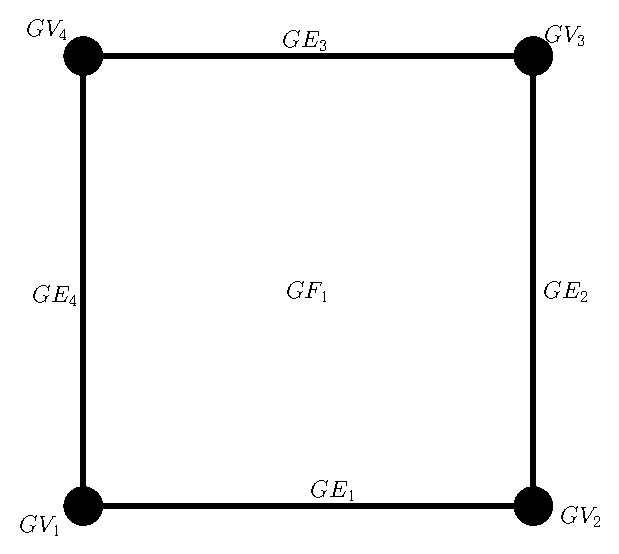
\includegraphics[scale=0.85]{figures/examplemodel}
      \end{center}
    \end{minipage}%
    \begin{minipage}{0.5\textwidth}
      \begin{center}
        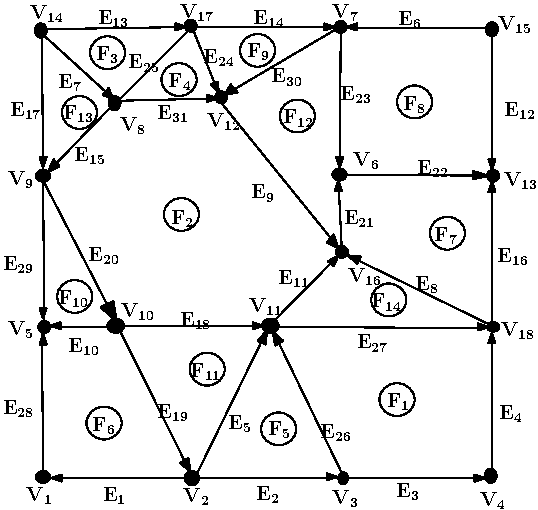
\includegraphics[scale=0.85]{figures/examplemesh}
      \end{center}
    \end{minipage}
  \end{center}
  \caption{Geometric model and a two-dimensional mesh of mixed elements of the model.}
\end{figure}

\newpage

File in F1 format:
\begin{verbatim}
MSTK 1.0
F1 18 31 14 0
vertices
0.00 0.00 0.00  0 1
0.33 0.00 0.00  1 1
0.66 0.00 0.00  1 1
1.00 0.00 0.00  0 2
0.00 0.33 0.00  1 4
0.66 0.66 0.00  2 1
0.66 1.00 0.00  1 3
0.16 0.84 0.00  2 1
0.00 0.66 0.00  1 4
0.16 0.33 0.00  2 1
0.50 0.33 0.00  2 1
0.40 0.84 0.00  2 1
1.00 0.66 0.00  1 2
0.00 1.00 0.00  0 4
1.00 1.00 0.00  0 3
0.66 0.50 0.00  2 1
0.33 1.00 0.00  1 3
1.00 0.33 0.00  1 2
edges 
2 1    1 1
2 3    1 1
3 4    1 1
4 18   1 2
2 11   2 1
15 7   1 3
14 8   2 1
18 16  2 1
12 16  2 1
10 5   2 1
11 16  2 1
15 13  1 2
14 17  1 3
17 7   1 3
8  9   2 1
18 13  1 2
14 9   1 4
10 11  2 1
10 2   2 1
9 10   2 1
16 6   2 1
6 13   2 1
7 6    2 1
17 12  2 1
8 17   2 1
3 11   2 1
11 18  2 1
1 5    1 4
5 9    1 4
7 12   2 1
8 12   2 1
faces edge
4  3 4 -27 -26            2 1
6  18 11 -9 -31 15 20     2 1
3  25 -13 7               2 1
3  31 -24 -25             2 1
3  2 26 -5                2 1
4  -28 -1 -19 10          2 1
4  16 -22 -21 -8          2 1
4  22 -12 6 23            2 1
3  -30 -14 24             2 1
3  -10 -20 -29            2 1
3  19 5 -18               2 1
4  9 21 -23 30            2 1
3  -15 -7 17              2 1
3  27 8 -11               2 1
attributes
velocity
VECTOR
3
MVERTEX
18
0 1    0.0  0.0  0.0
0 2    3.3  0.0  0.0
0 3    6.6  0.0  0.0
0 4   10.0  0.0  0.0
0 5    0.0  3.3  0.0
0 6    6.6  6.6  0.0
0 7    6.6 10.0  0.0
0 8    1.6  8.4  0.0
0 9    0.0  6.6  0.0
0 10   1.6  3.3  0.0
0 11   5.0  3.3  0.0
0 12   4.0  6.6  0.0
0 13  10.0  6.6  0.0
0 14   0.0 10.0  0.0
0 15  10.0 10.0  0.0
0 16   6.6  5.0  0.0
0 17   3.3 10.0  0.0
0 18  10.0  3.3  0.0
diffusity
TENSOR
3
MFACE
14
2 1    1.0 10.0 2.0
2 2    1.0 10.0 2.0
2 3    1.0 10.0 2.0
2 4    1.0 10.0 2.0
2 5    1.0 10.0 2.0
2 6    1.0 10.0 2.0
2 7    1.0 10.0 2.0
2 8    1.0 10.0 2.0
2 9    1.0 10.0 2.0
2 10   1.0 10.0 2.0
2 11   1.0 10.0 2.0
2 12   1.0 10.0 2.0
2 13   1.0 10.0 2.0
2 14   1.0 10.0 2.0
\end{verbatim}


\newpage
File in R1 format:
\begin{verbatim}
MSTK 1.0
R1 18 0 14 0
vertices
0.00 0.00 0.00  0 1
0.33 0.00 0.00  1 1
0.66 0.00 0.00  1 1
1.00 0.00 0.00  0 2
0.00 0.33 0.00  1 4
0.66 0.66 0.00  2 1
0.66 1.00 0.00  1 3
0.16 0.84 0.00  2 1
0.00 0.66 0.00  1 4
0.16 0.33 0.00  2 1
0.50 0.33 0.00  2 1
0.40 0.84 0.00  2 1
1.00 0.66 0.00  1 2
0.00 1.00 0.00  0 4
1.00 1.00 0.00  0 3
0.66 0.50 0.00  2 1
0.33 1.00 0.00  1 3
1.00 0.33 0.00  1 2
faces vertex
4  3 4 18 11              2 1
6  9 10 11 16 12 8        2 1
3  14 8 17                2 1
3  8 12 17                2 1
3  2 3 11                 2 1
4  1 2 10 5               2 1
4  6 16 18 13             2 1
4  6 13 15 7              2 1
3  7 17 12                2 1
3  5 10 9                 2 1
3  2 11 10                2 1
4  12 16 6 7              2 1
3  9 8 14                 2 1
3  11 18 16               2 1
attributes
velocity
VECTOR
3
MVERTEX
18
0 1    0.0  0.0  0.0
0 2    3.3  0.0  0.0
0 3    6.6  0.0  0.0
0 4   10.0  0.0  0.0
0 5    0.0  3.3  0.0
0 6    6.6  6.6  0.0
0 7    6.6 10.0  0.0
0 8    1.6  8.4  0.0
0 9    0.0  6.6  0.0
0 10   1.6  3.3  0.0
0 11   5.0  3.3  0.0
0 12   4.0  6.6  0.0
0 13  10.0  6.6  0.0
0 14   0.0 10.0  0.0
0 15  10.0 10.0  0.0
0 16   6.6  5.0  0.0
0 17   3.3 10.0  0.0
0 18  10.0  3.3  0.0
diffusity
TENSOR
3
MFACE
14
2 1    1.0 10.0 2.0
2 2    1.0 10.0 2.0
2 3    1.0 10.0 2.0
2 4    1.0 10.0 2.0
2 5    1.0 10.0 2.0
2 6    1.0 10.0 2.0
2 7    1.0 10.0 2.0
2 8    1.0 10.0 2.0
2 9    1.0 10.0 2.0
2 10   1.0 10.0 2.0
2 11   1.0 10.0 2.0
2 12   1.0 10.0 2.0
2 13   1.0 10.0 2.0
2 14   1.0 10.0 2.0
\end{verbatim}

\section{Example program}

NOTE: This program is included in the distribution.


\begin{verbatim}
#include <stdio.h>
#include <stdlib.h>
#include "MSTK.h"
#include "test.h"

int main(int argc, char *argv[]) {
 int i, idx, idx2, ok, edir, nv, ne;
 double xyz[3];
 char meshname[256];
 Mesh_ptr mesh;
 MVertex_ptr v;
 MEdge_ptr e;
 MFace_ptr f;
 GEntity_ptr gent;
 List_ptr fedges;
  

 if (argc == 1) {
   fprintf(stderr,"Usage: %s meshfilename (without .mstk extension)\n",argv[0]);
   exit(-1);
 }

 /* Initialize MSTK - Always do this even if it does
    not seem to matter in this version of MSTK */

 MSTK_Init();

 /* Load the mesh */

 strcpy(meshname,argv[1]);
 strcat(meshname,".mstk");

 mesh = MESH_New(UNKNOWN_REP);
 ok = MESH_InitFromFile(mesh,meshname);
 if (!ok) {
   fprintf(stderr,"Cannot find input file %s\n\n\n",meshname);
   exit(-1);
 }

 /* Print some info about the mesh */

 nv = MESH_Num_Vertices(mesh);
 for (i = 0; i < nv; i++) {
  v = MESH_Vertex(mesh,i);

  /* Basic info */
  printf("\n");
  printf("Vertex: 0x%-x   ID: %-d   ",v,MV_ID(v));
  
  /* Classification w.r.t. geometric model */
    
  if (MV_GEntDim(v) == -1)
    fprintf(stderr,"Unknown Classification\n");
  else {
   printf("GEntID: %-d   GEntDim: %-d\n",MV_GEntID(v),MV_GEntDim(v));
   if ((gent = MV_GEntity(v)))
     printf("Model entity pointer: 0x%-x\n",gent);   
  }

  /* Coordinates */
  MV_Coords(v,xyz);
  printf("Coords: %16.8lf %16.8lf %16.8lf\n",xyz[0],xyz[1],xyz[2]);
 }

 idx = 0;
 while (f = MESH_Next_Face(mesh,&idx)) {

  /* Basic info */
  printf("\n");
  printf("Face: 0x%-x   ID: %-d   ",f,MF_ID(f)); 
  
  /* Classification w.r.t. geometric model */

  if (MF_GEntDim(f) == -1)
   fprintf(stderr,"Unknown Classification\n");
  else {
   printf("GEntID: %-d   GEntDim: %-d\n",MF_GEntID(f),MF_GEntDim(f));
   if ((gent = MF_GEntity(f)))
    printf("Model entity pointer: 0x%-x\n",gent);
  }
  printf("\n");

  /* Edges of face */
  fedges = MF_Edges(f,1,0);
  ne = List_Num_Entries(fedges);
  printf("Edges: %-d\n",ne);
  printf("Object       ID     GEntID  GEntDim   Vertex IDs\n");
  idx2 = 0; i = 0;
  while (e = List_Next_Entry(fedges,&idx2)) {
   edir = MF_EdgeDir_i(f,i);
   if (edir) 
    printf("0x%-8x    %-8d %-8d     %-1d       %-d  %-d\n",
           e,ME_ID(e),ME_GEntID(e),ME_GEntDim(e),
           MV_ID(ME_Vertex(e,0)),MV_ID(ME_Vertex(e,1)));
   else 
    printf("0x%-8x    %-8d %-8d     %-1d       %-d  %-d\n",
           e,-ME_ID(e),ME_GEntID(e),ME_GEntDim(e),
           MV_ID(ME_Vertex(e,0)),MV_ID(ME_Vertex(e,1)));
   i++;
  }
  printf("\n");
  List_Delete(fedges);
 }

 if ((natt = MESH_Num_Attribs(mesh))) {

   fprintf(stderr,"Attributes on the mesh:\n\n");
   
   for (i = 0; i < natt; i++) {

     attrib = MESH_Attrib(mesh,i);

     attentdim = MAttrib_Get_EntDim(attrib);

     /* Won't print out edge, face and region based attributes
        but the code should be quite similar */

     if (attentdim != MVERTEX) continue;
     
     fprintf(stderr,"Attribute Number %-d\n",i+1);

     MAttrib_Get_Name(attrib,attname);
     fprintf(stderr,"Name: %-s\n",attname);

     atttype = MAttrib_Get_Type(attrib);
     switch(atttype) {
     case INT:
       fprintf(stderr,"Type: Integer\n");
       break;
     case DOUBLE:
       fprintf(stderr,"Type: Double\n");
       break;
     case VECTOR:
       fprintf(stderr,"Type: Vector\n");
       break;
     case TENSOR:
       fprintf(stderr,"Type: Tensor\n");
       break;
     default:
       fprintf(stderr,"Unrecognizable or unprintable attribute type\n");
       continue;	
     }

     switch(attentdim) {
     case MVERTEX:
       fprintf(stderr,"Applicable to vertices only\n");
       break;
     case MEDGE:
     case MFACE:
     case MREGION:
     case MALLTYPE:
       /* Won't print out edge, face and region based attributes
          but the code should be quite similar */
       continue; 
     default:
       fprintf(stderr,"Unrecognized entity type\n");
       continue;
     }

     ncomp = MAttrib_Get_NumComps(attrib);
     fprintf(stderr,"Number of components: %-d\n",ncomp);

     switch(attentdim) {
     case MVERTEX:
       idx = 0;
       while ((v = MESH_Next_Vertex(mesh,&idx))) {
         if (MEnt_Get_AttVal(v,attrib,&ival,&rval,&pval)) {
           fprintf(stderr,"V %-d: ",MV_ID(v));
           switch (atttype) {
           case INT:
             fprintf(stderr," %-d\n",ival);
             break;
           case DOUBLE: 
             fprintf(stderr," %-lf ",rval);
             break;
           case VECTOR: case TENSOR:
             rval_arr = (double *) pval;
             for (k = 0; k < ncomp; k++)
       	fprintf(stderr," %-lf ",rval_arr[k]);
             break;
           default:
             break;
           }
           fprintf(stderr,"\n");
         }
       }
       break;
     case MEDGE: case MFACE: case MREGION: case MALLTYPE:
       /* Skipped code to print out attributes for all other
          entity types but it is almost identical */
       break;	
     default:
       break;
     } /* switch (attentdim) */

   } /* for (i = 0; i < natt) */
   
 } /* if (Mesh_Num_Attribs(mesh)) */
  
 /* Write out a copy of the mesh */

 strcpy(meshname,argv[1]);
 strcat(meshname,"-copy.mstk");
 MESH_WriteToFile(mesh,meshname,F1);

 /* No need to delete a mesh if program ends right afterwards */

 MESH_Delete(mesh);
 return 1;
}
\end{verbatim}

\section{Acknowledgements}

This work was performed under the auspices of the National Nuclear
Security Administration of the US Department of Energy at Los Alamos
National Laboratory under contract No. DE-AC52-06NA25396 with partial support
from the Advanced Simulation Capability (ASC) program.

This manual has been reviewed by LANL and deemed suitable for unlimited
release (LA-UR-04-0878). MSTK has been reviewed by LANL and deemed suitable
for unlimited distribution (LA-CC-04-010). MSTK is distributed under
an LGPL open-source license.

\end{document}
